\documentclass[12pt, letterpaper,oneocolumn]{article}
\usepackage[margin=1in, letterpaper]{geometry}
\usepackage[toc,page]{appendix}
\usepackage{float}
\usepackage{amsmath}
\usepackage{amsthm}
\usepackage{amsfonts}
\usepackage{amssymb}
\usepackage{amsrefs}
\usepackage{fancyhdr}
\usepackage{pgfplots}
\usepackage{parskip}
\usepackage{unicode-math}
\usepackage{titlesec}
\usepackage{listings}
\usepackage{color}
\usepackage{booktabs}
\usepackage{circledsteps}
\usepackage{outlines}
\usepackage{hyperref}
\usepackage{cite}
\usepackage{url}
\hypersetup{
    colorlinks=true,
    linkcolor=red,
    filecolor=magenta,
    urlcolor=cyan,
}

\definecolor{dkgreen}{rgb}{0,0.6,0}
\definecolor{gray}{rgb}{0.5,0.5,0.5}
\definecolor{mauve}{rgb}{0.58,0,0.82}

\lstset{
	frame=tb,
	language=C++,
	aboveskip=3mm,
	belowskip=3mm,
	showstringspaces=false,
	columns=flexible,
	basicstyle={\small\ttfamily},
	numbers=none,
	numberstyle=\tiny\color{gray},
	keywordstyle=\color{blue},
	commentstyle=\color{dkgreen},
	stringstyle=\color{mauve},
	breaklines=true,
	breakatwhitespace=true,
	tabsize=4
}

\setlength\tabcolsep{14pt}

\titleformat*{\section}{\large}

\pgfplotsset{compat=1.17}

\setlength\parskip{10pt}

\pagestyle{fancy}
\rhead{Stephen Szwiec}
\lhead{BIOL492 Directed Research Writeup}
\title{BIOL492 Directed Research Writeup}
\author{Stephen Szwiec}
\date{\today}

\begin{document}
	\maketitle

	\thispagestyle{fancy}
	\tableofcontents
	\newpage
	\begin{abstract}
	The creation of programmed and scripted tools for biological data extraction and analysis remains an ongoing effort in the field of bioinformatics. Delivering high-throughput analysis for plant breeding programs is a unique subset of of this, given agronomic improvement program usage of this data to make critical workflow decisions. To facilitate such a program, the curation and navigation of databases and related tools is a continual process, with heterogeneous information networks, including high-performance computing (HPC), used in developing new crop germplasm. In Summer 2020, I worked with Bandillo Lab of North Dakota State University as it launched an effort to document processes, to engineer systems, and to improve use of HPC and machine learning resources.
	\end{abstract}

	\section{System Description}
	At NDSU Bandillo Lab, research is conducted using pea (\textit{Pisum sativum}), chickpea (\textit{Cicer arietinum}), and lentil (\textit{Lens culinaris}) to develop these pulse crops into cultivars suited to the \textit{terrior} of the northern plains region, and to improve the agronomically valuable phenotypes for these crop plants, including yield and protein content. The program is currently an 11 year-workflow, with each phase of testing performed in parallel across several test sites spanning the climate and soil basis of North Dakota \cite{NDdawn}. In this process, the lab harnesses the genetic biodiversity of the germplasm collections of affiliated organizations as starter genetic material \cite{coyne}. These accession lines, which consist of previously developed cultivars, divided by market class \cite{peaagro} \cite{lentilagro}, are used to create an initial parental $P$ cross between these two recombinant inbred lines in a randomized block with repetition in a greenhouse environment. A subsequent cross of the \textit{filial} $F_1$ generation repeats this randomized block breeding to generate variance in the population. Agronomically viable phenotype data is taken from both in the field and from quantitative chemical analysis of seeds yielded \cite{tpg2}. From generation $F_2-F_5$, phenotypic selection of nursery plants funnels the top-performing blocks from the first trials into a single plant selection per block. From generation $F_6-F_9$, observations on crop output yield factors and resistances to both biotic and abiotic stressors are taken, and phenotype data is analyzed using analysis of variance (ANOVA) \cite{dagenlie} and best linear unbiased predictors (BLUPs) \cite{blup} for the phenotype data set taken. Finally, at the $F_{10}-F_{11}$ generation, statewide testing confirming the phenotype values of the germplasm and full sequencing complete the agronomic selection process.

	\begin{center}
		\begin{figure}[H]
			\includegraphics[width=\linewidth]{selection_workflow.png}
			\caption{\textbf{Agronomic Selection Workflow} this diagram shows a simplified process workflow diagram for the lab, with agronomic selection occurring over 11 generations of crosses, and trials steps taken. Image used with permission, originally by Nanoy Bandillo (2020).
}
		\end{figure}
	\end{center}

	This program performs with a large data overhead, and consists of a heterogeneous network of information technologies with various deployment configurations. In May 2020, Bandillo Lab had phenotype data stored for the last 15 years, relating over 200 accession lines for pea, chickpea, and lentil, related to documenting the agronomic selection process. No networked or database system was in use for the management of genotype data, despite the core importance of this data to the project. The system was largely the legacy of a previous principal investigator at NDSU for pulse agronomics, and a cybersecurity attack in 2019 had encrypted notes from the previous team's process documentation.

\begin{center}
	\begin{figure}[H]
			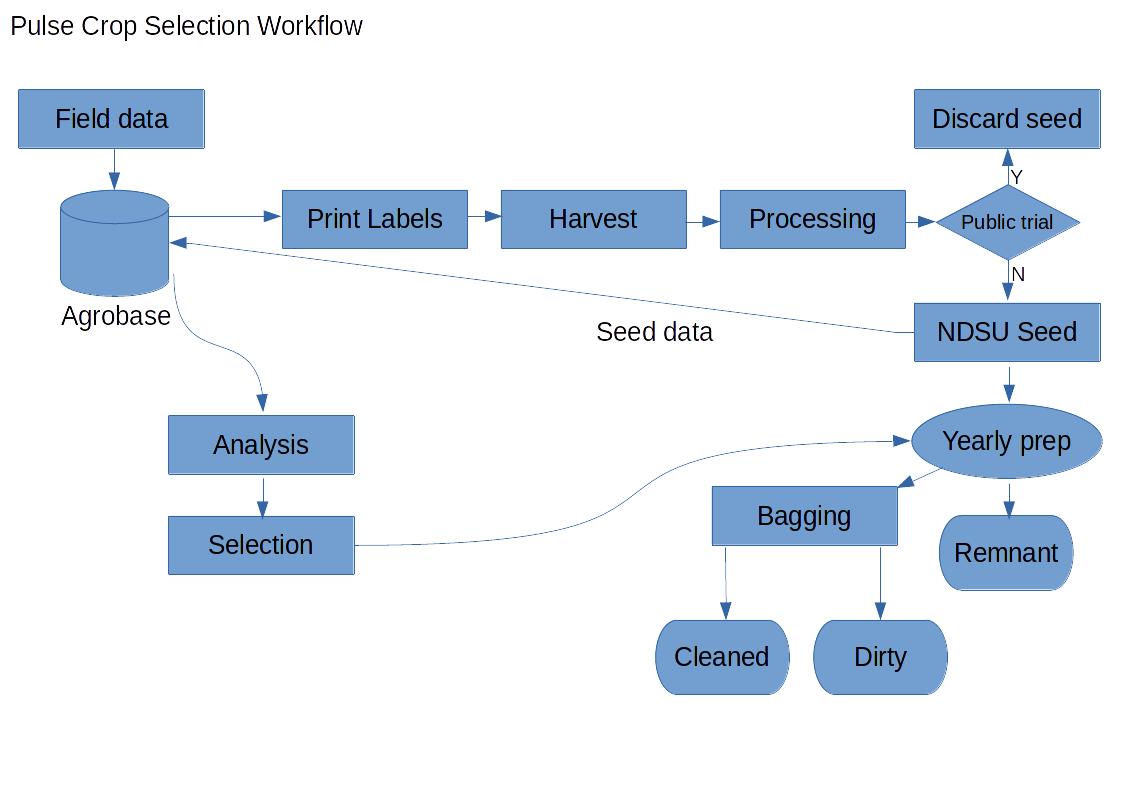
\includegraphics[width=\linewidth]{processing_workflow.png}
			\caption{\textbf{Field Trial Processing Workflow} this diagram shows a simplified process workflow diagram for field work per experiment, in which field trial organisms are analyzed, their seeds inventoried and processed, and the internal usage of database programs to facilitate this.}
		\end{figure}
		\end{center}

	\section{Agrobase Audit}

	\subsection{Introduction}
	In May 2020, the Bandillo Lab at NDSU performed an audit of the stored phenotype data. Agrobase\textregistered (Agronomix Inc., Winnipeg, Canada) is a closed-source phenotype database system offering experiment management and statistical analysis for agronomic data, and is used at NDSU across all of the agronomics and plant sciences programs. Primarily a GUI front-end to Microsoft SQL server, the Agrobase software provides a managed schema and templating system, and allows for data saved to have ANOVA performed in an automated fashion. This software has a prominent role at NDSU's plant science research, and falls under the purview of the Breeding Pipeline Database Management team; however, data of each breeding science team is individually managed by that same team.

	\subsection{Data Analysis}
	The database schema of Agrobase was studied to better understand the internal operations of the database system and to learn how to identify the outlying and anomalous data in Agrobase. For this task, a Windows 10 virtual machine was spun up as a test environment, into which both Agrobase software and Microsoft SQL Server were installed.

	A full database dump of the Agrobase server was performed using a Microsoft SQL API call made to the Agrobase server, where a local copy of the Agrobase database was created using the same schema using Microsoft PowerShell. This reverse-engineered schema was then studied to understand the distribution of data within the database system, and a visual representation of this schema was generated to better study information flow through the system as a reverse engineering of the processes undertaken by the program.

\begin{center}
	\begin{figure}[H]
		\includegraphics[width=\linewidth]{diagramEXP01.png}
		\caption{\textbf{Agrobase database schema} this diagram shows the highly linked nature of database tables within Agrobase, where treatments, experiments, experimental design, names, and raw data related to one agronomic line entry are spread across several tables.}
	\end{figure}
\end{center}

After study of this database schema to understand how then information was being saved across the system, a series of scripts were written to identify abandoned experiments, erroneous data entry, and experimental outliers. These scripts were developed referencing internal NDSU Research Extension Center document "Data Collection and Reporting Protocols, Revision 9 (2019)" (authored by Hannah Worral) which identified agronomic traits for the experimental datasets and typical reported data per trait. These scripts were run per agronomic trait for both pea, chickpea, and lentil data sets. Example SQL code of the scripts created are included in \textbf{Appendix A}, and these tools were used to extract information from the database in an efficient manner using a connection to the server within the virtual machine.

	\subsection{Findings and Actions Taken}
	Study of the Agrobase database schema showed that raw experimental data (including numeric data) was saved into Agrobase as character strings, and then presented to the user as a particular datatype, the definitions for which were saved in another table. This allowed for erroneous data to accumulate, as no datatype checking was applied as an input validation, which prevented non-numeric data input when not using the GUI interface.

	The audit of the Agrobase pulse crop database for abandoned experiments found that 58 chickpea experiments, 109 lentil experiments, and 244 pea experiments had no relevant agronomic data whatsoever, and could be removed from the database and archived for recording purposes to save system resources.

	Outlier identification audit script found a number of outliers for agronomic trait information, but also found erroneous entries (for instance, pea test weight with negative numeric values.) All outliers were compiled into a report for review by Bandillo Lab team members, with a report of lines which had reported yield and protein outliers four standard deviations above the mean compiled into a separate report for rapid agronomic improvement of those lines.

	Furthermore, steps were also taken to rectify erroneous data in Agrobase, either specifying that the particular data was instead lost or removing experiments for which no experimental data was found. All activities were logged and this log was presented to the Breeding Pipeline Database Management (BPDM) team \cite{BPDM}. These corrections allowed not only for improved database performance in the case of archiving abandoned experiments, but also allowed for new and subsequent experimental ANOVA analyses to better reflect their true experimental findings by removing erroneous data from the set.

	\section{Database Nomenclature Revision}

	\subsection{Introduction}
	After conclusion of the Agrobase audit, audit findings concluded that further action would need to be taken, as experiment nomenclature stored in the database had shifted over time into a number of styles. To allow for easier development in the future, a new harmonized nomenclature for pea, chickpea, and lentil was created.

	\subsection{Methodology}
	Working within the Bandillo Lab team, and in coordination with the BPDM team, interviews were conducted with plant breeders to understand the schema of information hierarchy used within the program, and what information was relevant to the program. It was determined that the nomenclature for the Pulse program for use with Agrobase and other database tools would need to be a standardized schema for interoperability with a number of APIs. The schema would need to be nominally human-readable and machine-searchable by use of regular expressions, such that the code would not overlap and always uniquely identify data and research assets across the program. Furthermore, this system would need to cover the breadth of experimental trials performed, and be accepting of retained unknown experimental data from the legacy system. After revision, experiments in process were recorded using this system. Full text of nomenclature developed from these methods available as \textbf{Appendix B}.

	\subsection{Future Work}
	While the nomenclature has been revised moving forward, future work includes scripted renaming of experiments in the database, and creating an index of these changes to harmonize these changes across all data in the program.

	\section{Genome-Wide Agronomic Selection - parallelization for HPC clusters}

	\subsection{Introduction}
	Genomic selection (GS) uses genome wide markers to predict breeding values \cite{gwas} rather than considering the discrete molecular biology components individually, a more inferential approach to identifying the causes of variance between populations can be performed by taking the imputed matrix of only the single nucleotide polymorphism (SNP) matrix of the differences between genotypes. This method is underpinned by the understanding of genetic gain over a given time, known as the Breeder's Equation \cite{lush2013animal}, given as:

	$$R=\frac{ir\sigma_{A}}{y}$$

	Where $R$ is gain in a quantifiable trait over time, with $i$ as selection intensity parameter, $r$ as accuracy value of selection, with additive standard deviation of genetic variances $\sigma_{A}$, for a given $y$ years. Having better prediction models, and performing earlier selection through genotype rather than by phenotype, allow agronomic researchers to maximize genetic gain on polyphenic traits.

	By performing training using machine learning models with Bayesian inference on a genome-wide association study (GWAS) \cite{Poland2015}, qualitative prediction of a phenotype from any given genotype can be prepared given some smaller training population. Such a model would be system in the form:

	$$Y_{ijk} = \mu + G_i + T_j + R_{k(j)} + e_{ijk}$$

	Where the observed quantitative phenotype $Y_{ijk}$ value is given by the system for the training data phenotype mean $\mu$, genotypic effect matrix $G_{i}$, random trial effect $T_{j}$, for $R_{k(j)}$ replication effects nested within a trial, with some residual error $e_{ijk}$. This model would also produce a heritability $H^2$ estimate \cite{Poland2015}, in the form:

	$$H^2 = \frac{\sigma^2_G}{\sigma^2_G + \sigma}$$

	Taken together, these predictions, heritability estimates, and residual error provide for actionable summary statistic data for agronomic improvement programs. Additional predictability of models can be achieved with the application of subpopulation structure as a weighted variable within the prediction models \cite{Soysubpop}.

	During the Summer of 2020, data analysis work on both genome-wide association study (GWAS) and on population substructure for a set of 482 accessions of field pea was performed in preparation of the recently-published article "Harnessing genetic diversity in the USDA pea (Pisum sativum L.) germplasm collection through genomic prediction." \cite{pea_diversity}. Data and findings from this publication have been republished with permission from its authors. The following provides more detail on the data science approaches used in preparation of this publication, and presents the same summary statistics as findings.

	\subsection{GWAS Data Analysis}
	Data analysis was performed as a scripted head-to-head training of machine learning models, with creation tasks on the NDSU CCAST Thunder2 super-computing cluster, using the R language \cite{R-lang} and running on Red Hat\textregistered Enterprise Linux\textregistered release 7.6 (Linux kernel 3.10.0), and utilized free and open source libraries, including The GNU coreutils \cite{GNU}, tassel5 \cite{tassel5}, and OpenPBS \cite{OpenPBS}.

	Pea genotype data for accessions was received in variant call format \cite{vcf}, and a script \textbf{Appendix C.1} was used to generate a numeric genotype SNP matrix. This genotype matrix was then used with phenotype data from experiments of the same accession to train the rrBLUP \cite{rrBLUP}, GAUSS \cite{GAUSS}, PLSR \cite{pls}, ELNET \cite{glmnet}, RF \cite{RF}, and AVE \cite{BGLR} models. heritability and accuracy tests were also performed. The script \textbf{Appendix C.2} also uses parallelization of these model training loops across a pool of compute cluster nodes, made available through the PBS script \textbf{Appendix C.3}. This parallelization was performed with doParallel in R \cite{doparallel} and utilized 24 CPU cores (Intel \textregistered Xeon \textregistered Gold 6140 @ 3.7Ghz) and 5GB of memory on the CCAST Thunder2 cluster for computation, requiring 11 minutes to process through the data.

	\subsection{Pea Population Structure}
	Data analysis of pea population structure was performed using ADMIXTURE \cite{admixture} using a 5-fold Quick Newton/Block validation for log likelihood of $k={1-10}$ subpopulations. Processing proceeded on NDSU CCAST Thunder2 cluster with 70 threads and 16GB of memory, and processing took 6 hours to complete.

	\subsection{Results}
	\subsubsection{Phenotypic heritability and correlation}
	The heritability for plant height was 0.81, with an average height of 74cm. Pods per plant had a heritability estimate of 0.50 with a mean of 18 pods per plant and ranged from 15 to 23 pods per plant. Days to maturity had a mean of 104 days with an estimated heritability of 0.51. Seed yield per hectare ranged widely from 1734 to 4463 kg/ha with a mean yield of 2918 kg/ha and a heritability value of 0.67. The number of pods per plant was highly and positively correlated with seed yield. Correlation estimation also suggested seed yield was positively correlated with plant height (PH), days to maturity (DM), days to first flowering (DFF). For summary statistics, see \textbf{Appendix C.4}.

	\subsubsection{Comparison of predictive ability of different genomic selection models} No single model consistently performed best across all traits that we evaluated. Predictive abilities from different models performed similarly, although slight differences were observed, likely due to existing trait complexity. For DFF, the highest predictive ability was obtained from PLSR and ELNET (0.57). The genomic selection model using rrBLUP resulted in the highest predictive ability for the number of seeds per pod (0.30), days to maturity (0.46), and seed yield (0.35). Gaussian kernel exhibited the highest predictive ability for plant height (0.52). The highest predictive ability for pods per plant was obtained through ELNET (0.27). For full detail,  see \textbf{Appendix C.5}.

	\subsubsection{Determining optimal marker density} To evaluate the increasing number of SNPs, we used the genomic prediction model with the highest predictive ability for a particular trait. For example, as PLSR provided the highest predictive ability for days to first flowering, we used this model to predict days to first flowering. In general, predictive ability increased with an increasing number of markers. The highest reported predictive ability was for the number of seeds per pod (0.30) at 30K markers. Pods per plant, plant height, and harvest date obtained the highest predictive ability when all ~31K markers were utilized. We got prediction accuracy for seed yield at 20K markers (0.41) compared to the rest marker density.

	\subsubsection{Population structure and prediction}
	Population structure analysis with ADMIXTURE yielded a strong inflection point at $k=7$, giving high likelihood of there being 7-8 ancestral subpopulations within the USDA pea germplasm. Based on >60\% ancestry, each accession was classified into eight subpopulations $(k=8)$. Using ADMIXTURE, we obtained eight subpopulations.

\begin{center}
	\begin{figure}[H]
		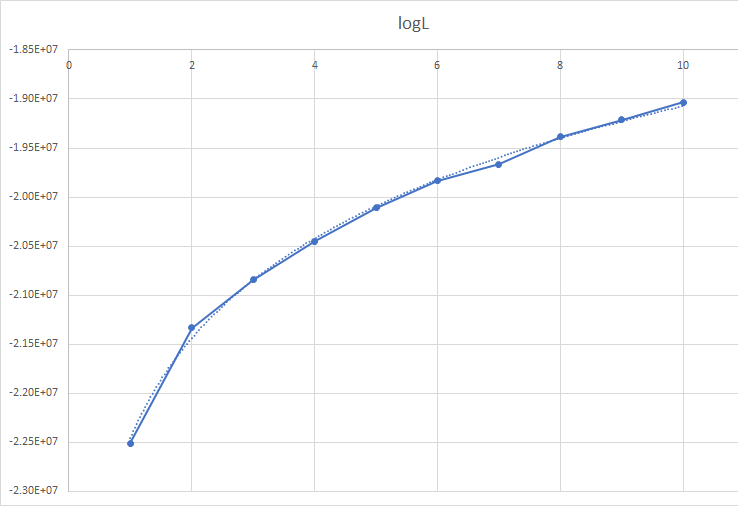
\includegraphics[width=\linewidth]{logLplot.png}
		\caption{\textbf{ADMIXTURE log likelihood} Results from ADMIXTURE analysis of pea accession SNPs using 5-fold QN/Block verification, X-axis showing number of subpopulation clusters, and Y-axis showing log likelihood convergence point of the algorithm.}
	\end{figure}
\end{center}

	Population structure explained some portion of the phenotypic variance, ranging from 9-19\%, with the highest percentages observed for plant height (19\%) and seed yield (17\%). Using either ADMIXTURE or PCA to account for the effect due to population structure, we improved the predictive ability. We observed a 6\% improvement for days to first flowering and 32\% for seed yield compared with models that did not account for population structure.

        We also performed within-subpopulation predictions. Presented here are the predictive abilities	for subpopulations 5, 7, and 8, as they had at least 40 entries. Subpopulation 8 had the highest predictive ability for days to first flowering (0.68), plant height (0.33), days to maturity (0.43), and seed yield (0.37). The highest predictive abilities for the number of seeds per pod (0.40) and pods per plant (0.12) were obtained from subpopulation 7. Notably, predictive ability was generally higher when all subpopulations were run in the model compared to when predictions were made within subpopulations.

	\section{Seed Inventory System Design}

	\subsection{Introduction}
	The adoption of the Internet as a platform for digital transformation within organizations had led to a greater sophistication of organization processes, allowing for real-time data sharing for internal and external users. The creation of integrated data services, in the form of various database-enabled applications, has allowed for a greater speed of processes, for a decreased cost of services provided, and for a greater capacity for quantitative decision-making through data analytics. In this paper, a web application and related organizational processes are described for the modernization of a seed inventory system, providing for a lean supermarket system with double-entry accounting. The case studied to arrive at this system is the NDSU Pulse Crops Breeding Program at the North Research Extension Center. This document will describe the current state of the seed inventory system, detail the changes made, provide a description of the database schema to be used, and finally describe the technological tools used to achieve these changes.

	August 2020, Bandillo Lab performed a transformative change to the processing of internal seed inventories. An ergonomic and usability study of the current system was performed and a kaizen process revision was performed, with a full proposal for a new seed inventory arising from this revision.

	\subsection{Description of System}
	At pilot site NDSU Minot North Central Research Extension Center (NCREC), seeds are divided by line and by experiment, and these seeds are kept in both envelopes and bags for the coming years. Bagged seeds are kept in a warehouse area: 300 inches in length and 196 inches in width (16.33ft x 25ft, or 4.97m x 7.62m), and these bags are kept in 42gallon (158L) plastic bins. Seeds in envelopes are otherwise stored in plastic trays in an adjacent room of the same warehouse. The database for this inventory system is kept on Agrobase, although the seed inventory module for Agrobase is not currently loaded. If a researcher would like to find a specific seed within the current system, that researcher would look at their computer, write down or print output from Agrobase, then find their seed based on this output.

	\subsection{Kaizen Audit Findings}
	The physical inventory system is both spatially wasteful, with seeds stacked into plastic bins, and is also a labor intensive and ergonomically brutal system to maintain, with the size of bins not allowing for quick repositioning and causing repetitive motion strain (stooping, lunging motions needed to find seed in bins). Furthermore, Agrobase tends toward being counter-intuitive for seed inventory: it is difficult to differentiate clean and dirty seed, years, experiment runs, etc. from seed inventory. This compounds to making tracking and auditing where specific seed comes from very difficult, and has no easy way to increment/decrement seeds from system. The system was overall found to be a blocking factor, wasting the time and effort of the people working with the system, and could easily be improved in this regard. Finally, the current system is not conducive for informed decision making about the seeds in inventory. This system should be replaced to not only eliminate ergonomic and usability bottlenecks, but also to provide a system which is informative, economic, and auditable.

	\subsection{Changes Made}
	The smallest immediate change was to implement a supermarket system inspired by the work of Taiichi Ohno \cite{ohno1988toyota} for all seeds otherwise kept in bins in the primary storage area to reduce the ergonomic load of the site. A physical organizational schema was devised using a floor plan of the area, and implemented as follows.

	Furthermore, a proposal for a future system was put into place. This includes a feasibility study of available open-source platforms for development.

	\subsection{Required Components}
		\begin{outline}[enumerate]
			\1 A wireless internet connected computer with monitor, such as a laptop, capable of running a modern browser and a free USB port (RasPi+monitor+battery, Chromebook, netbooks, etc.)
			\1 A wheeled trolley cart for moving inventory, with the top platform having space reserved for the computer system
			\1 USB connected plug-and-play bar-code scanner
		\1 Shelving units with bar-coded labels
		\1 Seed bags or envelopes with bar-coded labels
	\end{outline}
	\subsection{Physical Organization}

	\begin{center}
	\begin{figure}[H]
	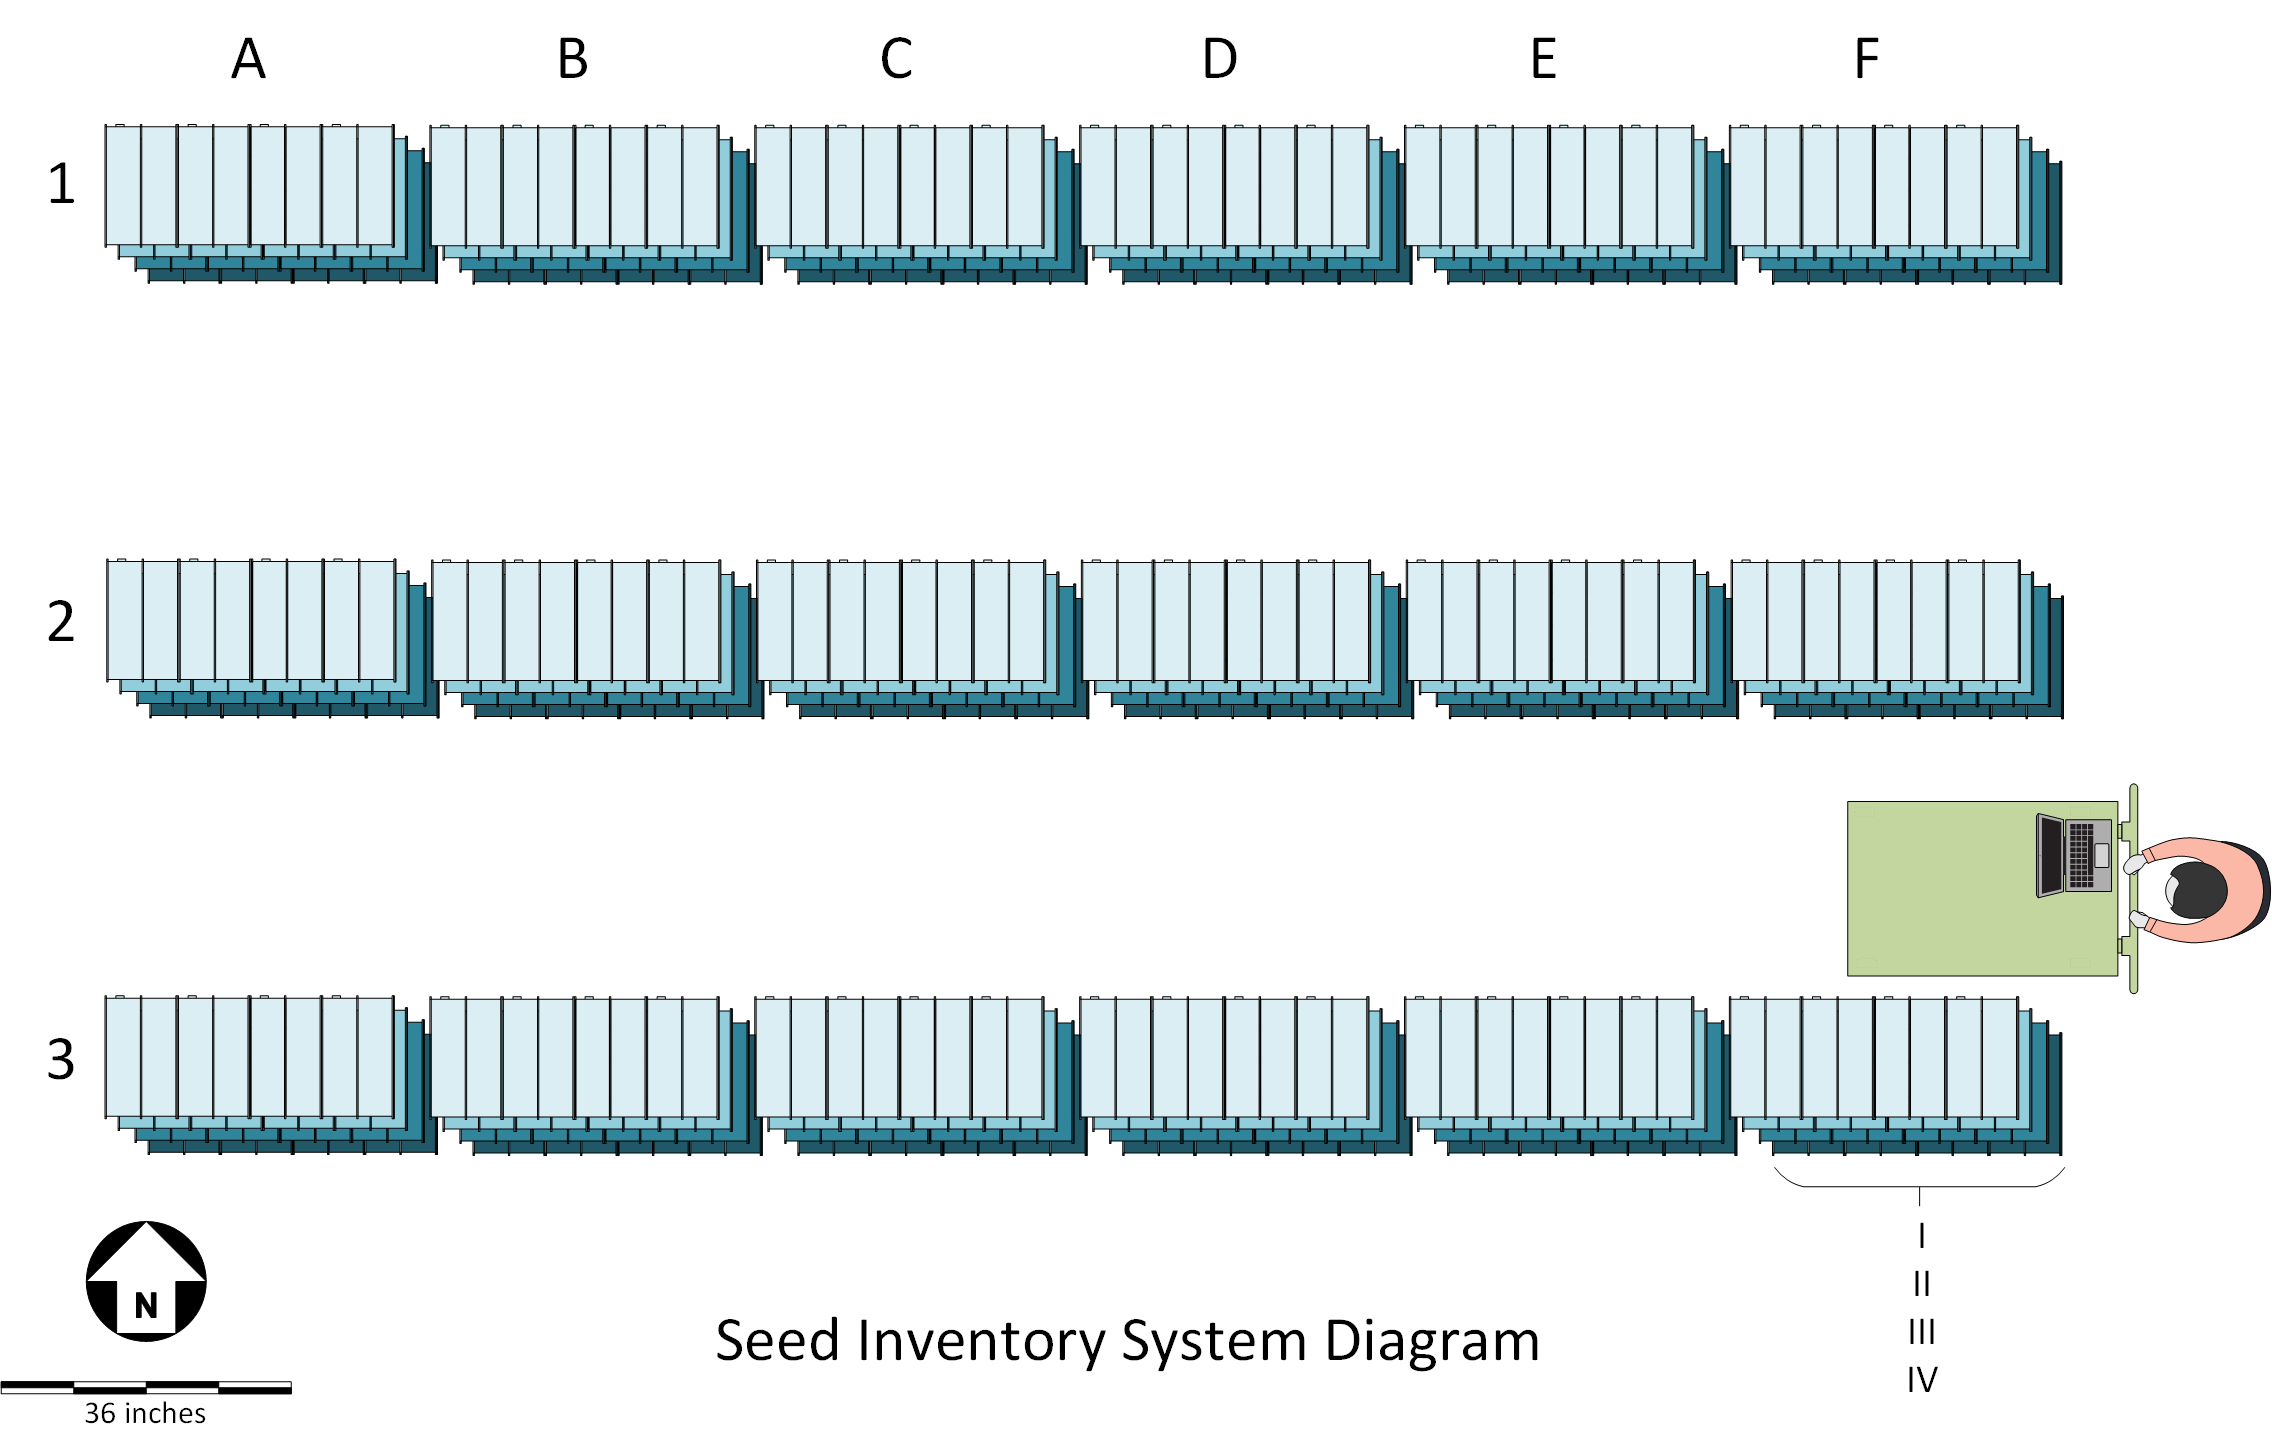
\includegraphics[width=\linewidth]{SeedInventoryLayout.png}
	\caption{\textbf{Seed Inventory Layout} this diagram shows the implemented inventory layout at Minot NCREC pilot location. Figure shows 4 tiered shelving units with orientation reflecting the ordering schema of the overall system, and is built with the ergonomics of agricultural workers in mind. After successful launch with pilot, this system was re-implemented across other research sites.}
		\end{figure}
\end{center}


	\begin{outline}[enumerate]
	\0 The first component of the seed inventory system is to have a consistent physical organization structure, which is defined as the following:
		\1 All seeds are to be kept on shelving units, such that no bag or envelope-tray is kept higher than 60inches (152cm) to prevent ergonomic strain, workplace accidents, and wasted effort retrieving equipment.
		\1 All shelving units are to be physically organized in the following manner:
			\2 Shelving units are to be kept in rows and columns when possible, such that columns align East to West, and rows align North to South, and such that the aisles between shelving units also run East to West.
			\2 Shelving units are to be placed such that the aisle between shelving units has adequate spacing for people to move through the aisle abreast of each other. At least 36inches (91cm) are to be allotted to each aisle.
			\2 Shelf labeling schema
				\3 each column of shelving will receive a letter, \textbf{A-Z} onward to \textbf{AA-ZZ} if necessary.
				\3 each row of shelving will receive a number, onward from \textbf{1}.
				\3 each shelf, top to bottom, will receive a roman numeral, onward from \textbf{I}.
		\1 Shelving which cannot be arranged in rows and columns for safety or usability purposes should nonetheless use a similar grid arrangement to labeling schema: if shelves line the perimeter of a room, then each shelf can be considered one column, with each shelving unit a singleton member of its row: \textbf{A1, A2, A3}, etc.
		\1 Each shelf is to have affixed one bar-code per working side of the shelf, and this label also gives a human readable full name of that shelf in Column-Row-Shelf format. For example, the unit of the third column, second row, and forth shelf would be labeled \textbf{C2-IV}.
		\1 All seeds should be labeled, with primary defining characteristics printed on a label, including a machine readable bar-code with the seed name on both sides.
	\end{outline}

	\subsection{Proposed Future System}
	\begin{center}
	\begin{figure}[H]
	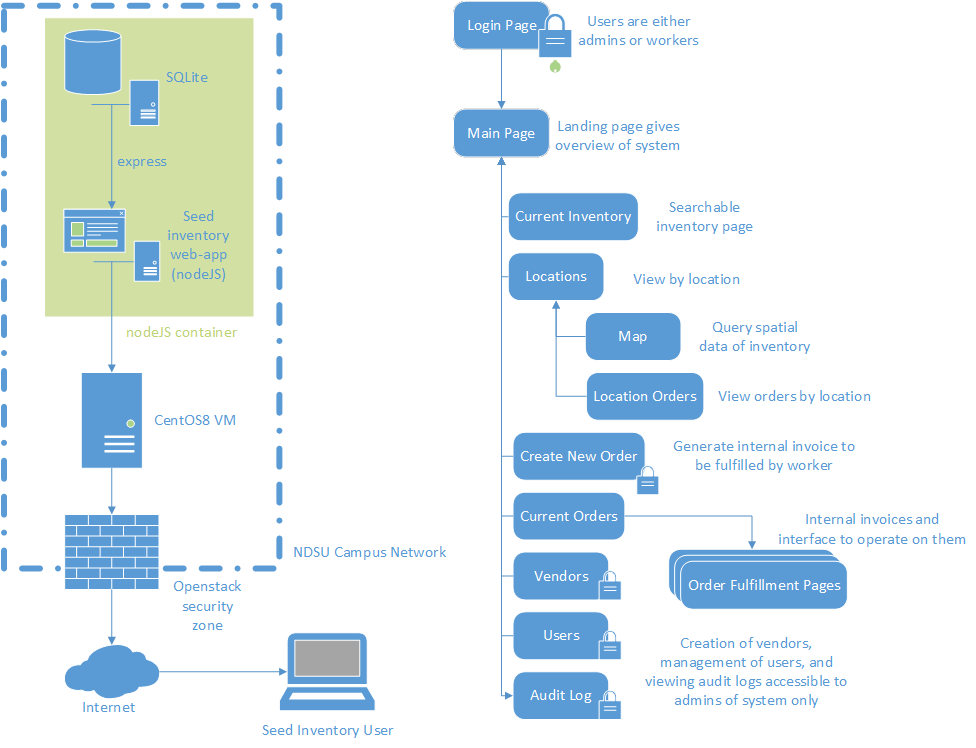
\includegraphics[width=\linewidth]{SeedInventoryManagementSystem.png}
	\caption{\textbf{Seed Inventory Layout} on left: network infrastructure diagram showing the seed inventory system alone within a larger NDSU-managed IT environment communicating to web interface user through the Internet. On right: seed inventory user presentation of web application pages, with locks showing administrative pages otherwise not shown to workers fulfilling orders.}
		\end{figure}
\end{center}


In addition to the physical organization, the seed inventory is to be enabled through a client-server database program, which is hosted on a web-server and made available to users through a browser. This program will be constructed using available FOSS, and will itself be free and open source. \\
The following are a list of enabling FOSS technologies to be used to create the software component of this system:
		\subsubsection{GNU Affero General Public License version 3}
		Developed by the Free Software Foundation (FSF) and Dr Richard Stallman, the GNU General Public License (GPL) is a freely-applicable software license which allows the user of that software to run, study, share, and modify the software for any purpose. Rather than retaining strict copyright, it allows for authorship of the software creator to be retained while distributing in a free and open source manner, in a system known as 'copyleft'. More specifically, the GNU Affero General Public License version 3 (AGPL) provides a legal framework for the source code of a website to be offered over a network, allowing for the larger academic and programming communities to benefit from the inclusion of this software. The full text of the AGPLv3 is available at the GNU webpage \cite{GPLAffero}.
		\subsubsection{CentOS 8 GNU/Linux}
		The CentOS Project is a community-driven, free software project based around the GNU operating system and Linux kernel and is available to anyone on the CentOS webpage \cite{centos8}. This software distribution has several strengths, including receiving its upstream software updates from Red Hat Enterprise Linux, a wide number of available software packages, and community support.
		\subsubsection{Docker}
		Docker is a platform as a service (PaaS) system to deliver apps as containerized, lightweight, virtual systems. Utilizing the Linux container subsystem, Docker applications can be built and shipped as a container, such that the internal state of the app does not effect other running applications in the same environment, and the internal state of the app is fully described in code. This allows for a higher degree of security control than running services on bare-metal, allows for apps to scale for load balancing, and allows for predictable behavior of apps on all platforms. More information about Docker is available on the Docker webpage. \cite{docker}
		\subsubsection{SQLite}
		SQLite is a C-based SQL engine which provides for speed and high-reliability. This community-based project has created a system fully implementing all ACID properties and has provided its source code to the public domain. This system was chosen over similar systems such as PostgreSQL or MySQL due to its high speed, low overhead, and long-term support for the project. More information about SQLite is available on the project website. \cite{sqlite}
		\subsubsection{NodeJS}
		NodeJS, created by the OpenJS Foundation, is a server which listens for HTTP(S) requests and serves pages, much like any other web-server. Unlike Apache and nginx, NodeJS is fully built in JavaScript, and allows for client-side and server-side scripting to communicate seamlessly by using JS as a framework. This type of environment, called 'full stack JavaScript' allows for the creation of web-2.0 style web applications with low development overhead. This is made possible through `npm`, the package manager of NodeJS, which is at this time the largest software package repository in the world \cite{npm_state}. These packages can be used in any configuration to develop web applications using these frameworks.  More information about NodeJS and npm are available on the project webpage. \cite{nodejs}
		\subsubsection{Express}
		Express is a minimal and flexible web application framework, available in npm, which allows for the creation of Application Programming Interfaces (APIs). In other words, Express acts as a middleware between client-side events which happen in the user's browser, and the server-side handling of data, such as SQLite. Using Express, the pages of the site are saved as API calls, which cause different HTTP responses to be sent dynamically. As such, pages are built based on the information gathered from the database, and thus in sync without further human intervention, allowing the webpage to be a front-end to database operations. Full documentation and explanation of Express is available on their project webpage. \cite{express}
		\subsubsection{Angular}
		Based on previous work by Google on the npm package AngularJS, Angular is a FOSS web framework which can be used to create user interfaces which adapt to both mobile and desktop browsers. This system is modular and allows for the creation of websites which are as dynamic and responsive as desktop-based applications. Furthermore, Angular has been redeveloped from the predecessor AngularJS to eliminate security flaws, and has been developed with security as a primary concern. Documentation is freely available on their project webpage. \cite{angular}
		\subsubsection{Bootstrap}
		Bootstrap is the most popular HTML, CSS, and JS library currently in use, originally developed by Twitter as a framework to standardize user interface design. As a JavaScript framework, it works with Angular to provide prebuilt design elements, themes, and icons out of the box, allowing coders to focus on implementation rather than visual design. The Bootstrap project and examples are made available on their project webpage. \cite{bootstrap}
		\subsubsection{ngx-admin}
		A free and open source website administration panel, ngx-admin is another user interface web framework selected for this project. It implements a familiar panel design layout with features useful to database operations, including form validation, chart generation, the creation of data tables, and authentication. These features combined with the open and extensible nature of the framework, will save on development costs: rather than reinventing the wheel, only the functional features of the code will have to be implemented using prebuilt design elements. A demo of the various design elements provided is available as a web application. \cite{ngx-admin}
		\subsubsection{Mocha}
		Mocha is a test framework for NodeJS applications, which allows for serialization of testing during continued development for building automated unit tests of pages produced. Test driven development (TDD) allows for the creation of a test framework to be run at each change pushed to code, allowing for the automation of testing and for clear feedback to be given to the developer. In this way, bugs are catalogued during development with a lower overhead given to hiring UI/UX testers, or burdening the developer with manually checking each element of the program. Mocha and information about it is available on the project webpage. \cite{mocha}
		\subsubsection{Github}
		GitHub is a website which allows for the hosting of git-based software repositories at no cost \cite{git}, and provides a number of features and frameworks which allows for easier management of development operations. Available both as a web interface and as an API, GitHub provides storage and version control for code and a number of related tools. The current repository for the NDSU Pulse Crops program is located at project page Bandillo-Lab on Github, and all code produced for this application will reside there.
	\subsection{Database Schema}
	The database schema for this project is a data schematic, showing the relationships between information sets which will be stored in the database as tables. Using the framework provided by SQLite, this information will be used to provide content for the functional model of the application. \\

	\begin{center}
	\begin{figure}[H]
	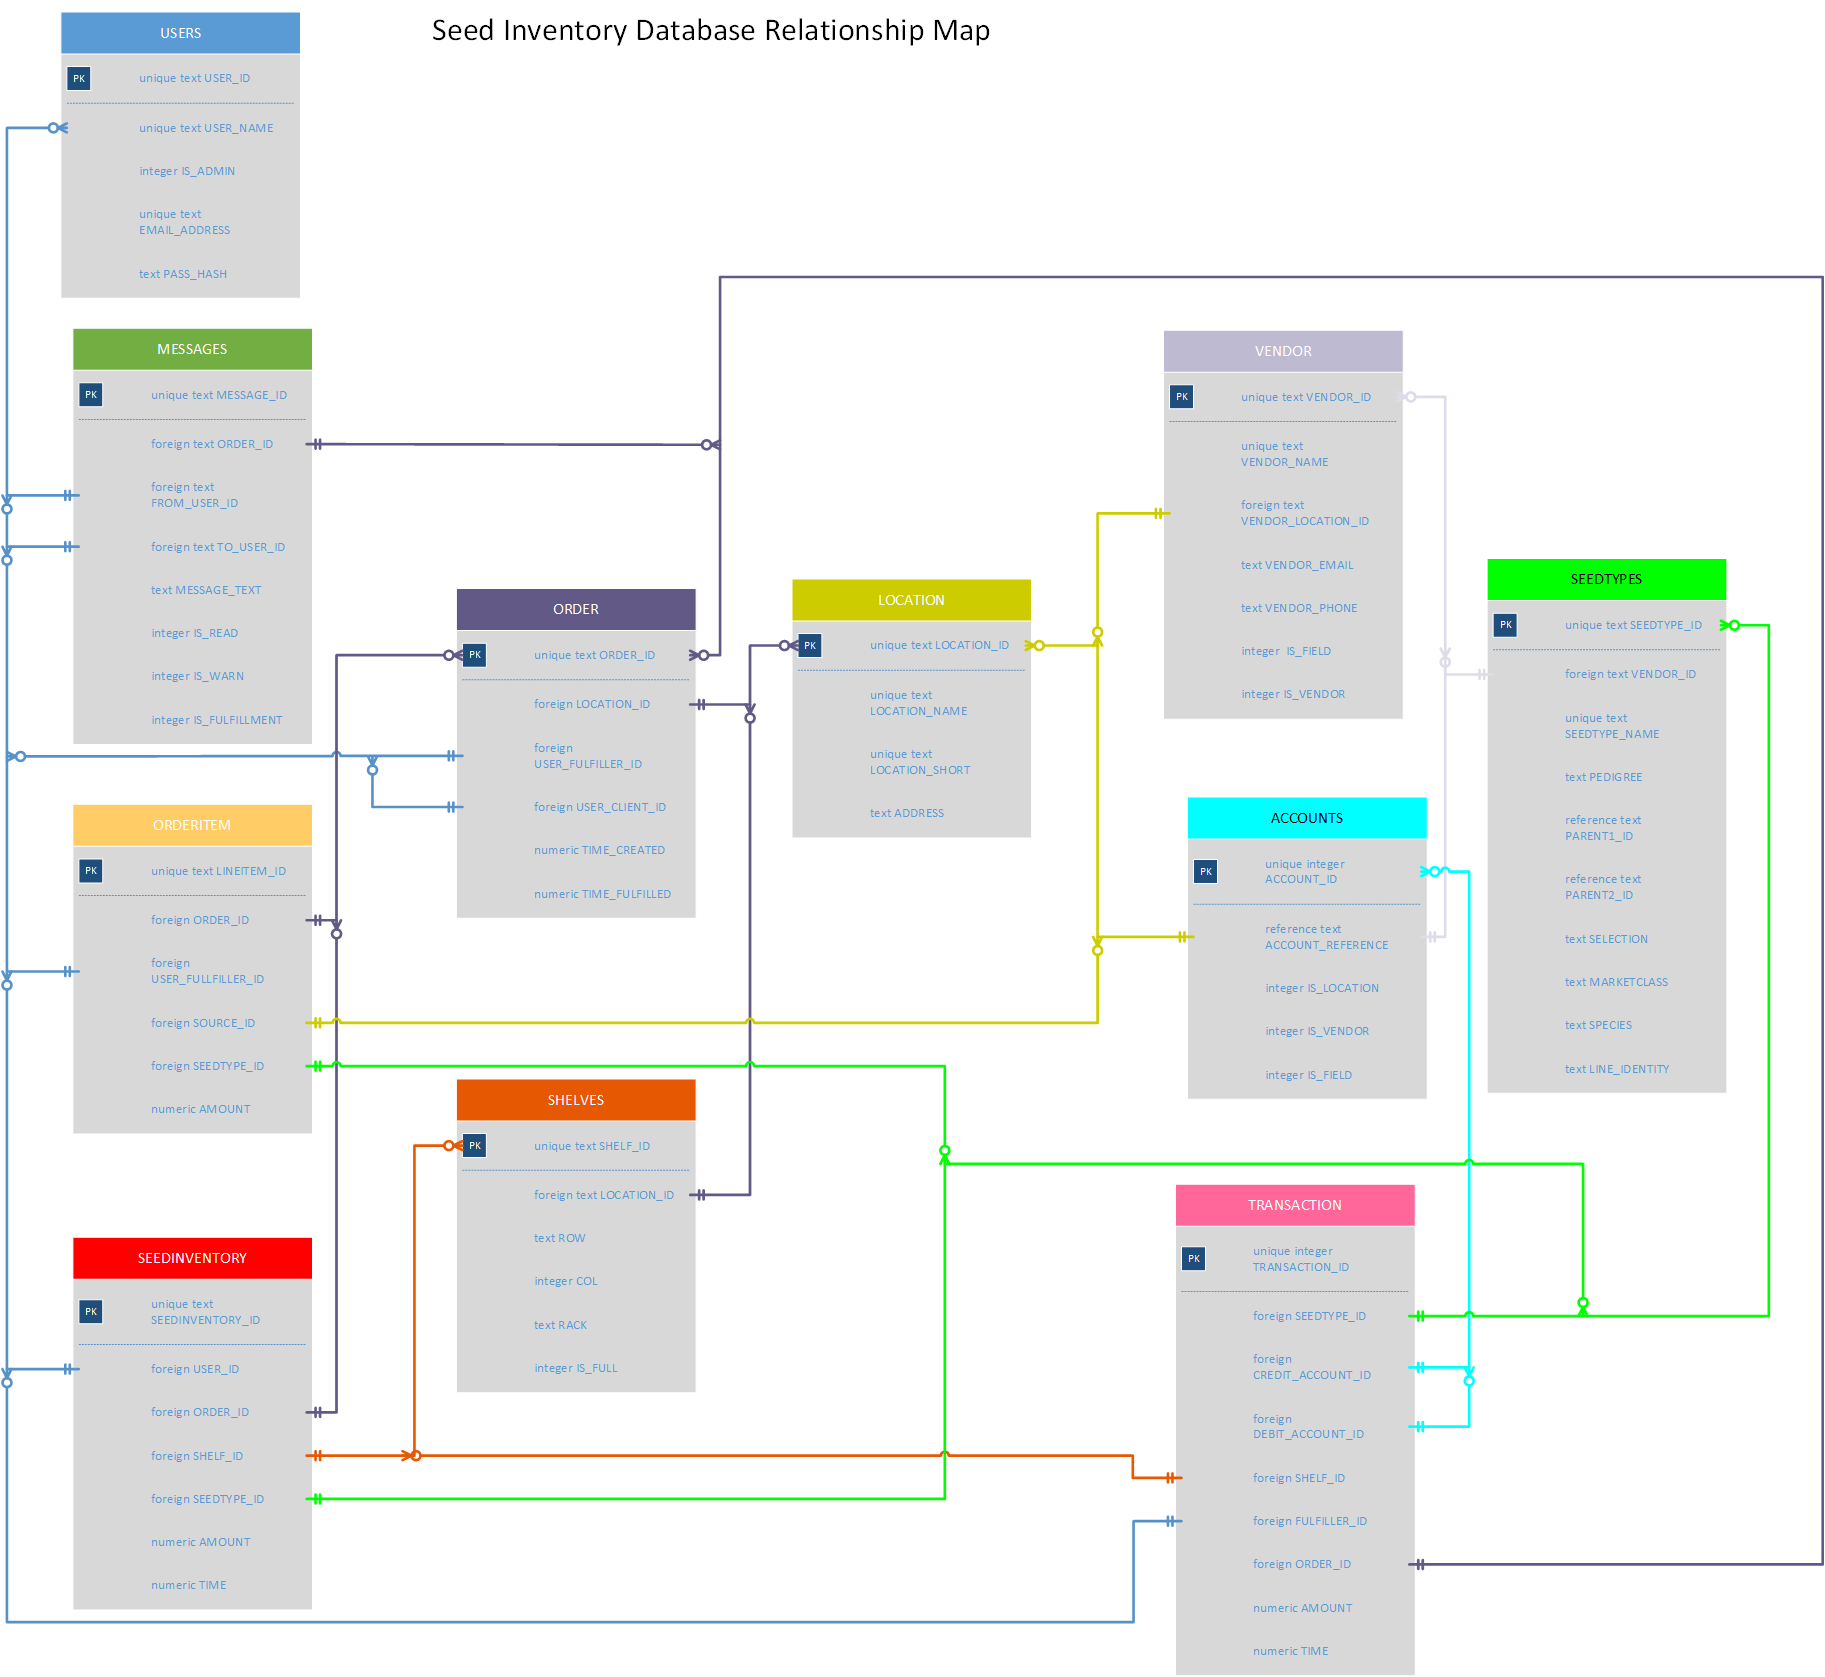
\includegraphics[width=\linewidth]{SeedInventoryDB.png}
	\caption{\textbf{Seed Inventory Database Schema} this diagram shows the database schema for the proposed system, with tables linked by inherited data flows via foreign keys to produce a stateful representation of the inventory system.}
		\end{figure}
\end{center}
	\textbf{Primary IDs} For both system security and for program flexibility, each row of each table will be given a system-side (rather than user-visible) unique primary key, which will be six randomized alphanumeric characters prefaced by a three character code based on its table membership, separated with an underscore. For instance, an ID for the USER table will be in the form \textbf{USR\_XXXXXX}. This nomenclature prevents cracking of database structure via sequential ID calls, and allows for for $62^6$, or over 56.8 billion database entries before the namespace is exhausted.
		\subsubsection{Users}
The USERS table contains all information about the current system users. This information is as follows: \\
\begin{outline}
	\1 A primary key unique alphanumeric text USER\_ID, with the three character prefix USR
	\1 A unique text USER\_NAME
	\1 An integer, 0 or 1, IS\_ADMIN, which provides differing privileges for administrator and worker user accounts
	\1 A unique text EMAIL\_ADDRESS, for future system email integration
	\1 A text PASS\_HASH, which will be the hashed password of the user (no plain-text passwords will be saved in the system). This field will be supplied by the Argon2 hashing algorithm, which is recommended by OWASP for all new applications. \href{https://cheatsheetseries.owasp.org/cheatsheets/Password_Storage_Cheat_Sheet.html}{[13]}
\end{outline}
		\subsubsection{Locations}
The LOCATIONS table contains information about locations where the seeds are to be stored, or placeholder locations of seed sources. These locations have the following properties: \\
\begin{outline}
	\1 A primary key unique alphanumeric text LOCATION\_ID, with three character prefix LOC
	\1 A unique text LOCATION\_NAME
	\1 A unique text LOCATION\_SHORT similar to the location abbreviations in Agrobase
	\1 A text ADDRESS
\end{outline}
	\subsubsection{Vendors}
Vendors are any possible source of seeds within the program, and include external vendors (such as private companies, other universities, or government bodies like the USDA) or internal sources (such as field activities, winter greenhouse, and other locations). The VENDOR table has the following properties:
\begin{outline}
	\1 A primary key unique alphanumeric text VENDOR\_ID, with three character prefix VND
	\1 A unique text VENDOR\_NAME
	\1 A foreign text VENDOR\_LOCATION\_ID, which will either be NULL for external vendors or a reference to another location in the program for internal vendors
	\1 A text VENDOR\_EMAIL which may be NULL
	\1 A text VENDOR\_PHONE which may be NULL
	\1 An integer IS\_FIELD, set to 1 if this vendor is a field, 0 otherwise
	\1 An integer IS\_VENDOR, set to 1 if this vendor is a literal external vendor of seed, 0 otherwise
\end{outline}
		\subsubsection{SeedTypes}
The SEEDTYPES table contains all information pertaining to stored types of seeds. This information is separate from the seed inventory itself, and as such each seed inventoried will have a seed type information set associated with it. SeedTypes have the following properties: \\
\begin{outline}
seed	\1 A primary key unique alphanumeric text SEEDTYPE\_ID, with three character prefix STP
	\1 A unique text SEEDTYPE\_NAME identifying the line
	\1 A foreign text VENDOR\_ID, associating the seed type with its source
	\1 A text PEDIGREE
	\1 A text PARENT1\_ID which can either be NULL or a reference to another row in the SEEDTYPE table
	\1 A text PARENT2\_ID which can either be NULL or a reference to another row in the SEEDTYPE table
	\1 A text SELECTION, detailing the selection phase of the seed
	\1 A text MARKETCLASS, detailing the market-class of this seed
	\1 A text SPECIES, detailing the species
	\1 A text LINE\_IDENTITY, for further internal association with line nomenclatures
	\1 A numeric THOUSAND\_SEED\_WEIGHT, describing the weight of 1000 seeds of this type
\end{outline}
	\subsubsection{Shelves}
The SHELVES table contains all information of shelves in the program. Shelves have the following properties:
\begin{outline}
	\1 A primary key unique alphanumeric SHELF\_ID, with three character prefix SLF
	\1 A foreign non-null text LOCATION\_ID, placing the shelf at a physical location in the program
	\1 A text COLUMN (A-Z,AA-ZZ)
	\1 An integer ROW (1-N)
	\1 A text STACK (I, II, III, etc.)
	\1 An non-null integer IS\_FULL, which is either 1 for a full shelf or 0 otherwise.
\end{outline}
	\subsubsection{Orders}
The internal logic of the system is based on the fulfillment of orders, which are internal invoices of planned changes to the inventory system. the ORDERS table can be thought of a list of orders for workers to fulfill on. The ORDERS table has the following properties:
\begin{outline}
	\1 A primary key unique alphanumeric ORDER\_ID, with three character prefix ODR
	\1 A foreign, non-null LOCATION\_ID referencing what site the order is for
	\1 A foreign, non-null USER\_CLIENT\_ID referencing the administrator creator of the order
	\1 A foreign USER\_FULFILLER\_ID, which is either NULL when an order is not fulfilled and otherwise a reference to the user who completed the order
	\1 A numeric non-null TIME\_CREATED
	\1 A numeric TIME\_FULFILLED which is initially null and timestamped at order completion
\end{outline}
		\subsubsection{OrderItems}
Rather than the converse, where Orders may have an unknown number of Order Items, all Order Items instead have a foreign key to its originator in Orders. The ORDERITEMS table contain these order items, which can each be thought of as a change requested for the seed inventory. The ORDERITEMS table has the following properties:\\
\begin{outline}
	\1 A primary key unique alphanumeric ORDERITEM\_ID, with three character prefix ITM
	\1 A foreign ORDER\_ID reference to its parent order
	\1 A foreign SOURCE\_ID which is a reference to  a LOCATION of either a vendor or another internal seed inventory location\\
	\1 A foreign SEEDTYPE\_ID detailing what type of seed to be moved\\
	\1 A numeric AMOUNT giving the count or weight of the order item, positive for additions to inventory and negative for seeds removed\\
	\1 A text UNIT giving the unit of the amount\\
\end{outline}
		\subsubsection{Messages}
The message system is a user interface element allowing for communication between users on the platform. These messages may be automatically generated (on order fulfillment, order creation) or be the result of a user's interaction with the system (a worker flags an order as having a problem). The MESSAGES table has the following properties:\\
\begin{outline}
\1 A primary key unique alphanumeric MESSAGE\_ID, with three character prefix MSG\\
\1 A foreign ORDER\_ID reference to its parent order, which may be NULL if no order is related to the message\\
\1 A foreign FROM\_USER\_ID referencing the sender of the message\\
\1 A foreign TO\_USER\_ID referencing the receiver of the message\\
\1 A text MESSAGE\_TEXT field\\
\1 An integer IS\_READ which is either 1 if the receiver has seen it, or 0 otherwise\\
\1 An integer IS\_WARN, which is ether 1 for priority messages, or 0 otherwise\\
\1 An integer IS\_FULFILLMENT, which is either 1 for fulfillment confirmations, or 0 otherwise\\
	\end{outline}

	\subsubsection{SeedInventory}
The seed inventory is the heart of the system and the primary goal of the system is to establish a granular command and control system over this information. The SEEDINVENTORY table is a list of all seeds in the inventory system, and has the following properties:\\
\begin{outline}
	\1 A primary key unique alphanumeric SEEDINVENTORY\_ID, with three character prefix SDI\\
	\1 A foreign USER\_ID referencing the user who placed the seed in its current spot\\
	\1 A foreign SHELF\_ID referencing the inventory item's current location\\
	\1 A foreign ORDER\_ID referencing the order which pulled the inventory item into the system\\
	\1 A numeric AMOUNT, a seed weight in grams\\
	\1 A text UNIT\\
	\1 A numeric TIME of when it was last modified\\
	\1 An integer IS\_DIRTY clearly marking whether the seed has been cleaned\\
\end{outline}

	\subsubsection{Accounts}
An account is an abstract entity created for the accounting purposes of the seed inventory system. Every location has an associated account, and this account is used to populate the information of the TRANSACTIONS table. the ACCOUNTS table has the following properties:\\
\begin{outline}
	\1 A primary key unique alphanumeric ACCOUNT\_ID, with three character prefix ACC\\
	\1 A foreign non-null LOCATION\_ID\\
	\1 A foreign VENDOR\_ID which is NULL for internal locations\\
	\1 An integer IS\_LOCATION for internal locations, which is 1 if the account describes an inventory location and 0 otherwise\\
	\1 An integer IS\_VENDOR, which is 1 if the account describes a literal vendor and 0 otherwise\\
	\1 An integer IS\_FIELD, which is 1 if the account describes a field activity and 0 otherwise\\
\end{outline}

	\subsubsection{Transactions}
A transaction is any change made to the inventory database across its entire life, and this is the 'general ledger' of what could be described as a double-entry accounting system. As changes are made to the inventory, it is credited or debited, and a corresponding, mirror-image debit or credit is applied to another account reflecting the movement of seeds across the system. This TRANSACTIONS table is used to provide auditing for the system, and as such is an indelible record for any given accounting period. This table will only reset in length at the end of a seed inventory audit, on date the table will be compressed and saved outside of the database. The TRANSACTIONS table has the following properties:\\
\begin{outline}
\1 A primary key unique alphanumeric TRANSACTION\_ID, with three character prefix TSN\\
\1 A foreign SEEDTYPE\_ID reference\\
\1 A foreign CREDIT\_ACCOUNT\_ID reference\\
\1 A foreign DEBIT\_ACCOUNT\_ID reference\\
\1 A foreign SHELF\_ID reference\\
\1 A foreign ORDER\_ID reference\\
\1 A numeric AMOUNT\\
\1 A text UNIT\\
\1 An integer IS\_DIRTY\\
\1 A numeric TIMESTAMP
\end{outline}
	\subsection{Functional Model and User Experience}
The overall user experience and functionality of the web application will be through the web browser and initially hosted at the Pulse Program webpage (https://pulse.ccast.ndsu.edu/). Upon navigation to this site, the user will be asked to login using their username and password. \\
Once the user has logged in, they will be taken to a landing: page, showing information including outstanding orders, recently fulfilled orders, and general system information at a glance. A top menu will display an icon, indicating any waiting messages for the user. On the left-hand side of the application, a collapsible menu will show the following options:\\

\begin{center}
	\begin{figure}[H]
	\includegraphics[width=\linewidth]{mockup.png}
		\caption{\textbf{UI/UX Proof of Concept Mockup} Generated from free and open source libraries previously mentioned, this proof of concept web interface was demoed for the lab members to demonstrate the layout, look, and feel of a fully implemented system.}
		\end{figure}
\end{center}

\begin{outline}
\1 \textbf{Home} the current page\\
\1 \textbf{Current Inventory} a table of all inventory, with drop down menus and text input elements used to search this table and narrow down information. This will include a button to export current view as a CSV.\\
\1 \textbf{Locations} a table view of all locations in the database, allowing selection of location to view more specific information for each and three additional functions\\
	\2 \textbf{Map} generate a map of the current inventory of a selected location \\
	\2 \textbf{Location Orders} view outstanding and fulfilled orders by location\\
	\2 \textbf{Location Inventory} similar to 'Current Inventory' view, but with the current location already selected\\
\1 \textbf{Current Orders} a queryable view of all current orders in sequence\\
	\2 \textbf{Order Fulfillment Pages} generated by and accessible by each outstanding order, provides a workflow for checking inventory items into or out of the database. Workers can scan bar-codes or key in item IDs to pull changes across the inventory system here.\\
The following additional pages will be available to administrator accounts:\\
\1 \textbf{Create New Order} generate an internal invoice to push changes to the inventory by selecting seed types, sources, and amounts using text boxes and drop down menus\\
\1 \textbf{Vendors} view, modify, create, and delete vendor information\\
\1 \textbf{Users} view, modify, create, and delete users\\
\1 \textbf{Audit Log} view and query the transaction-level log of the database, output as CSV, or generate an end-of-period audit to close the ledger and begin a new one\\
\1 \textbf{Import Data} import data into tables from external dataset: provides interfaces for import via CSV file or SQL connection, then shows changes to be made (allowing modifications).\\
\end{outline}

\section{Virtual Machine Environment Planning}

	\subsection{Introduction}
	Since the first full DNA sequencing by Sanger in 1977, a series of breakthroughs in genomic sequencing, taken together as Next Generation Sequencing techniques, has applied computation toward genomics problem sets. With the decrease in costs of information technology associated with laboratory data management, the decrease in costs to Next Generation Sequencing (NGS) technologies (far exceeding the rate of Moore's Law \cite{GSPcost}), and the wider availability of reference genomes available for use by plant breeders \cite{ensembl} \cite{phytozome} the implementation of a NGS platform 'in house' is more cost-effective and feasible than ever.

	The rationale for the creation of a genomics database platform for the Pulse Breeding Program at NDSU extends from the present state of research. At the present time, NDSU plant breeding programs purchase sequencing services from outside laboratory partners. This data, generated at a cost, is a valuable part of the breeding programs using it. Therefore, as an asset, the genetics data received from outside partners requires a data management system, which not only stores this data in a durable and highly-available manner, but also allows for analytics performed on this data, and keeps knowledge about the data within a managed system. Such a system would not only safeguard the investment made on this data, but also allow for improved usage of data integration of genomics datasets into continued development. Such a system would allow for plant breeders to leverage the vast number of free-and-open-source genomics software tools now available without the creation of ad-hoc systems for each experiment or program.

	In addition, by keeping genomics development within the platform, one can expect time-savings, as workflows become more routine and algorithms more optimized to the problem sets at hand. Moreover, such a platform would open up new possibilities for research, not only for the development of agronomic gains in researched species, but also for the development of new algorithms, tools, and methodologies for the same as new resources become available.

	Given the highly heterogeneous information environment and high throughput of lab data workflows, the management of information technology, and systems administration tasks have become part of the data science work done within laboratories today. Moving genomic data between HPC clusters, personal researcher computers, organization web-servers, and rented services requires programming interfaces and API calls. At the present time, the NDSU agronomics program does not have an integrated data platform for genomics data. The current database platform, while robust, is not fully featured enough for genomics, nor does its structure provide for an open platform for further internal development by researchers. Therefore, a technological solution to incorporate genomics research and techniques into the plant breeding pipeline should be explored. The first component of this would be the implementation of a genomics database.

	A feasibility study was conducted to provide recommendations and draft a proposal for a curated virtual environment which would initiate a genomics database platform at NDSU, these goals were expanded to incorporate the scope of the previously described seed inventory system as well. The goals of the implementation plan included in the proposal are as follows:

	\begin{outline}
		\1 Describe the problems currently faced by the pulse plant science team and provide for solutions within the scope of an information system.
		\1 Provide cost estimates, cost-benefits analysis, and alternative implementation plans for IT components of the system.
		\1 Summarize and provide a logical outline for eventual project management of the system.
		\1 Summarize and link to the various supporting documentation cited to arrive at these solutions.
		\1 Detail the major architectural design aspects of the system in greater detail, comprising:
		\2 \textbf{Functional Design} detail regarding major functional aspects of the system and how the system will access the information it needs from the information environment.
		\2 \textbf{Technical Design} detail regarding how the major components of the system will be implemented in hardware, software, networking, database, and policy.
		\2 \textbf{Confidentiality, Integrity, and Availability} will be discussed as a functional component within the scope of both these designs.
		\1 Detail the documentation to be generated during the systems design, development, testing, and deployment processes, including the anticipation for change management and revisions.
		\1 Act as an open and living document, allowing for comment and feedback to be provided.
	\end{outline}

	\subsection{Requirements}

	\subsubsection{Functional Overview}
At the present time, NDSU agronomics breeding outsources genetic
sequencing to outside laboratory partners, which perform sequencing for
sampled specimens. For this data to be made more useful to researchers,
a database platform is necessary to further explore and analyze the
relationships between different genomes and the variation between plant
genotype and phenotype data. The features which will allow for the
highest return on investment for the research community at NDSU would
include high data durability, high data availability, integration of a
knowledge management system, and genomics annotation and indexing.

\paragraph{1. Data Durability} The following features are defined as requirements for the new storage platform in regards to the durability of data housed such that:

\begin{itemize}
\item
  data integrity features in-file-system to ensure reliability for the
  data.
\item
  high I/O performance to enable better response to end users.
\item
  protection against data corruptions.
\item
  file system snapshots for quick online backups, which don't load the
  servers.
\item
  quota allocations per user.
\item
  hardware level redundancy and hot-swappable hardware.
\item
  off-site backup performed with both incremental and full backups.
\item
  automated backup and scheduled testing of backups with notifications.
\end{itemize}

\paragraph{2. Data Availability}
The following features are defined as requirements for the new storage
platform in regards to the availability of the data housed such that:

\begin{itemize}
\item
  continued availability during hardware or software failure built into
  the system via HA pair or cluster topology.
\item
  real-time compression to optimize storage and also achieve higher
  performance.
\item
  data should be agnostic to any front end or workstation OS, and be
  called via API for common tools already used by researchers (R,
  Python, etc.)
\item
  data should be usable for common bioinformatics and statistical use
  cases, including next-generation modeling and Machine Learning.
\item
  no single point of failure in systems hardware effects overall
  availability of data.
\item
  usage of mature, commodity hardware to ensure replacement of
  components in case of failure and high uptime.
\item
  proper access controls and strong encryption employed to ensure data
  is available within the organization and is not exposed to
  non-organization members, even when moved across third-party systems.
\item
  cold spare platform in place for disaster recovery.
\end{itemize}

\paragraph{3. Knowledge Management}
In the context of informatics, empirical observations, as the data of an information system, drive the creation of information, with the analysis and processing of data yielding scientific conclusions. The data stored is not an end onto itself, but is instead made useful by revealing its underlying structure through a series of processes, procedures, and methodologies. The imperative and descriptive knowledge, taken together as organizational knowledge, is itself a core competency of laboratory science. This drive to retain knowledge within organizations is challenged by the diverse yet related datasets within biological sciences and by the communication overhead of research team members performing work separated by time, space, and across disciplines. \cite{knowledge_management}

While extensive work has been done by NDSU for the creation of data management systems for phenotype data, there exists no knowledge management system for the retention of internal processes and methodologies related to processing this data. As genomic data management is included, the scale and complexity of data within the information system will increase, and with it, the value of a knowledge management system as a means to both facilitate collaboration and reporting between researchers, and to provide return on research investment as documented expert knowledge. With knowledge management, this knowledge also remains within the information system even when experts are not available. Therefore, in addition to the proposed data management system, it is a functional requirement of the new system to include a knowledge management system, which will allow researchers to produce documentation of processes, procedures, and methodologies and for this documentation to be managed with similar durability and availability requirements as the data stored.

\paragraph{4. Data Pre-processing}
Raw genomics data provided to NDSU breeding program is provided in FASTA/FASTQ format, which consists of both raw reads of sequences and comments provided per run. Even alone, this data presents a technical challenge to genetics-driven research \cite{EJ910}; however, the density of genetics sequence data is also an informatics challenge. For data to be useful to data-driven decision making, datasets must be both easily searchable and available for comparison. By default, both of these properties are difficult to obtain with the FASTA/FASTQ format, given both the density of data and the lack of context given to this data. For example, the whole-genome sequencing kept on reference by the NCBI for \emph{Pisum sativum} is 4.6GB of data when uncompressed, or over 61 Million lines of 80 character width text with description lines included \cite{pea_genome}. Mapping this raw genetic sequence into genes, regulatory mechanisms, introns, exons, phenotypes, etc. to determine the relationships which make the data useful both in systems biology and plant breeding is a primary challenge in bioinformatics as a practice. Two techniques to expose these relationships, and help to reduce the technical overhead necessary for researchers to interact with genetics datasets: genome annotation and genome indexing, taken together, serve to expose the most pertinent structures of genetics datasets for further study, and as such are valuable labor-saving tools and are functional requirements for the proposed system.

\subsubsection{Proposed System}

Having enumerated through the functional components necessary for genomics research, the following provides an overview of the software fulfilling the technical requirements which enable these functions. System design incorporated requested comments from NDSU BPDM and Bandillo Lab members.

\begin{center}
	\begin{figure}[H]
		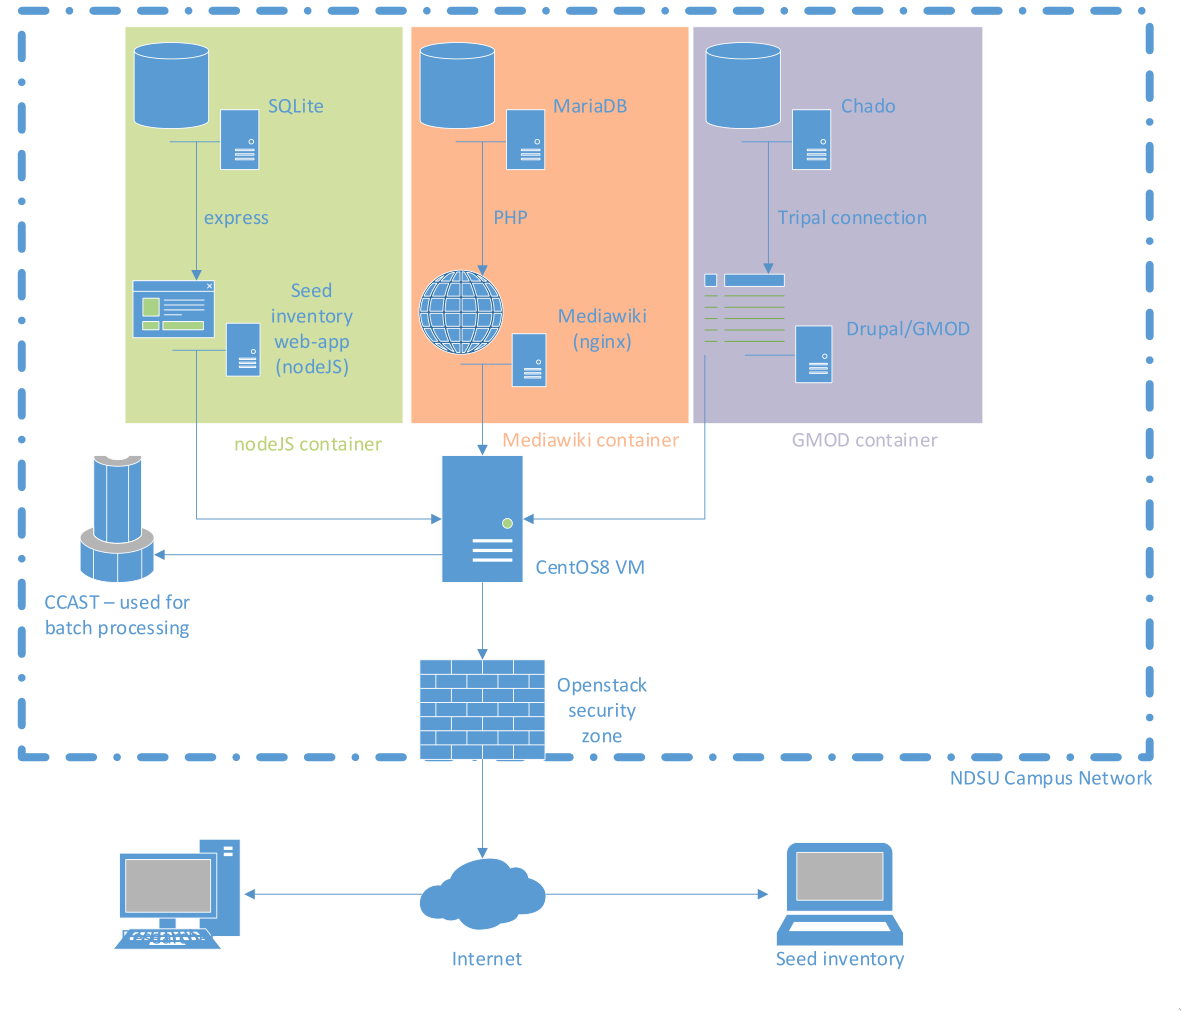
\includegraphics[width=\linewidth]{VMProposal.png}
		\caption{\textbf{Virtual Machine IT Environment} this diagram shows the three virtual machines identified as database applications useful to the breeding program's data analytics goals. At the present time, only the Centos host and the Mediawiki portion of this environment has been implemented, while the remaining have been approved for continued work.}
	\end{figure}
\end{center}

The system consists of an application host server running within the NDSU CCAST security zone of the NDSU network. This virtual machine consists of a Centos 8 image running on an Openstack \cite{openstack} virtual network, and is itself running Docker \cite{docker} to containerize application functionality. By leveraging the pre-existing network infrastructure of CCAST, this system can not only use the redundancy and fungibility of that system, but also allows for incredibly high throughput processing of openPBS scripted data science and machine learning tasks via the CCAST Thunder2 HPC cluster.

To fulfill the scope of the laboratory knowledge management system for genomic data processing, Mediawiki \cite{wiki:xxx} was chosen, with MariaDB \cite{mariadb} providing database back-end. Maintained by the Mediawiki Foundation, Mediawiki provides for a simple web application stack with builtin document revision history tracking and its own document formatting hypertext language, Wikitext,  allowing for detailed instructions and knowledge to be retained in the organization by researchers. By providing a private wiki instance, a shared location for scientists to share procedures, templates, and information is created. Furthermore, this repository also allows documentation of all work done for genomics database, allowing the system to become largely self-documenting.

As for the genomics database itself, review of current university best-practice confirmed that an instance of the Generic Model Organism Database system (GMOD) \cite{GMOD} would provide the needed functionalities of scripted data pre-processing, gene annotation, and gene indexing. Utilizing the free and open source Drupal content management framework, GMOD allows for parallel genomic data work-tasks via Chado, its database back-end, by scripting in BioPerl \cite{bioperl}.

As previously described, the final container running on the system is the seed inventory system, incorporating a nodeJS based web application providing researchers and agricultural workers access to a SQLite database system via express RESTful \cite{REST} middleware. As opposed to the other software, which will be taken from available open source packages, this inventory system will instead be built in-house to address the lack of free and open source inventory systems for plant breeders.

\subsubsection{Work Performed}

\paragraph{Cybersecurity Hardening}

	A guideline was developed using guidelines from USDA and FDA Cybersecurity Infrastructure Plan \cite{sipp}, NIST SP 800-53 Rev 5 \cite{nist}, and CIS benchmarks \cite{cis} to develop a hardening checklist, consisting of configuration changes from a base Centos 8 system running within NDSU CCAST. The entirety of these scripts and configuration modifications are available in \textbf{Appendix D}.

	\paragraph{Mediawiki implementation}
	In order to facilitate the change management overhead of continued systems improvements and implementations, a private wiki instance was used to document processes, policies, and proposal revisions. This system used Mediawiki running in a container inside of Docker, and a full documentation of the procedure for the creation of a lab wiki is in \textbf{Appendix E}

	\subsection{Future Work}
	At the present time, a virtual machine host and mediawiki implementation has been implemented in full. Future work on this system includes the creation of the seed inventory system web application as a free and open source Docker image, and the integration of GMOD for genomic data annotation and analysis.

	\section{Conclusions and Research Direction}
	The data science and statistical analysis tasks demonstrated in the course of research suggest that continued decreasing costs of high-throughput sequencing and phenotyping by sequencing technologies will, in turn, increase the network administration and systems administration tasks undertaken by bioinformaticians, statisticians, and data scientists. In addition, the size of genomic datasets and information density of genetic annotation data requires careful planning in the creation of robust and highly-available database systems to provide access to this data. The heterogeneous nature of the information network systems traversed during research also suggests that training in both management of information systems and cybersecurity training should also be pursued by data scientists and bioinformaticians as supplemental to and understanding of the field. Most tasks can be performed with free and open source software (FOSS) libraries. This body of FOSS code and its supporting documentation provides for custom analysis software pipelines and applications to be assembled from these libraries. However, with this comes increased overhead in time spent maintaining software and creating documentation for laboratory processes, workflows, and data output is of the utmost importance to data scientists to reduce costs from the creation of ad-hoc programming tools. Document management systems and knowledge management such as git and mediawiki are easy to implement and provide for a reduction in research time spent when used in a laboratory setting alongside more familiar database platforms, adding context and process awareness to data. Taken together, the frameworks and techniques presented here contribute to continued discovery of data analysis and management of information systems best practices, to be expanded upon.



	\newpage

	\begin{appendices}

		\section{Agrobase Audit}

		The following code were used to perform auditing of the Agrobase system.\\
		\subsection{Abandoned Experiment Identification}
		The following script was one of a series developed to identify abandoned experiments in the database, for which no experimental data was recorded. Three similar scripts were used, one each for the pea, chickpea, and lentil datasets. The script shown displays all abandoned experiments for the chickpea dataset. Note that metadata information of raw experiment data was saved across several tables.

		\lstset{language=SQL}
		\begin{lstlisting}
use chickpea
--select * from dbo.tre01; --this is the table that contains treatments varieties, populations, parents

--select * from dbo.exp01; --this table contains information about experiments

--select * from dbo.EXD01; --information related to experimental design keys

--select * from dbo.EXD02; --contains raw data for all traits

--select * from dbo.TRD01; -- contains the names of all the traits of experiments

--select * from PEA.dbo.VW_TreatTraitsWN; -- secret decoder ring for trait numbers

--select * from PEA.INFORMATION_SCHEMA.COLUMNS where COLUMN_NAME = 'TBENT1' order by TABLE_NAME ASC; --dump every table column name in the DB schema

declare @t_exp table (
	c_id int,
	c_year int,
	c_name varchar(50)
);

declare @t_data table (
	c_id2 int,
	c_data varchar(500)
);

insert into @t_exp (c_id,c_year,c_name ) select tbid,tbyear,tbname from dbo.exp01;
insert into @t_data (c_id2, c_data) select
	dbo.exd02.TBKEXPT,
	TBDATAC
	from dbo.exd02i
	where TBDATAC != ('-9.0');
delete from @t_data where c_data = '';
delete from @t_data where c_data like ('%-9%');


delete @t_exp
from @t_exp
inner join @t_data on c_id = c_id2
where c_id = c_id2;
select * from @t_exp
select * from @t_data order by c_data asc
		\end{lstlisting}

		\subsection{Outlier Identification}
		The following script was one of a series developed for outlier identification. This script identifies all non-null, non-missing entries four standard deviations from the mean for the 'test weight' (pounds per bushel) data for the lentil dataset. A different script was deployed for each of the agronomic traits described by Agrobase due to the peculiarities of string to numeric data conversion performed by Agrobase.

		\lstset{language=SQL}
		\begin{lstlisting}
use lentil;

--get metadata for the trait from the db
declare @trait int = 25;
declare @datatype char = (select TBFLD_TYPE from TRD01 where TBID = @trait);
declare @data_len int = (select TBFLD_LEN from TRD01 where TBID = @trait);
declare @data_dec int = (select TBFLD_DEC from TRD01 where TBID = @trait);
print @data_len;
print @data_dec;

--make a table in memory for exporting information
declare @t_exp table (
		c_id int,
		c_year int,
		c_name varchar(50),
		c_mean decimal(20,1),
		c_sigma float(5),
		c_outliers varchar(500)
);

--make a table in memory for storing raw plot data
declare @t_data table (
		c_id2 int,
		c_data decimal(20,0)
);

--populate the export table with information for all experiments which are not multiyear
insert into @t_exp (c_id,c_year,c_name ) select tbid,tbyear,tbname from dbo.exp01 where TBYEAR>0;

--populate the data table with non-null, non-garbage raw data for the trait selected
declare @script nvarchar(max);
set @script = N'select dbo.exd02.TBKEXPT, cast(cast(TBDATAC as float)as decimal(' + cast(@data_len as nvarchar(2)) + N',' + cast(@data_dec as nvarchar(20)) + N')) from dbo.exd02 where TBKTRAIT =' + cast(@trait as nvarchar(20));
insert into @t_data (c_id2, c_data) exec(@script);

delete from @t_data where c_data = NULL;
delete from @t_data where c_data = 0;
delete from @t_data where c_data like ('%-9%');

--remove any experiments which have no raw data whatsoever from the export table
delete from @t_exp
	where not exists(select NULL
		from @t_data where c_id2 = c_id);

--perform calculation of means and sigma values
declare @currentID int;

declare idx cursor local static read_only forward_only
for	select distinct c_id from @t_exp;

open idx;
fetch next from idx into @currentID;
while @@FETCH_STATUS = 0
begin
	update @t_exp set c_mean =
		(select avg(c_data)
		from @t_data where c_id2 = @currentID)
		where c_id = @currentID;
	update @t_exp set c_sigma =
		(select STDEV(c_data)
		from (
			select c_data
			from @t_data
			where c_id2 = @currentID)
		c_data)
		where c_id = @currentID;
	fetch next from idx into @currentID;
end;
close idx;
deallocate idx;

--calculate outliers
declare @i int = 1;
declare @index int = 0;
declare @rowCount int = 0;
select @rowCount = COUNT(0) from @t_exp;
declare @stdRange float = 4.0;
declare @lower decimal(20,1);
declare @upper decimal(20,1);
declare @mean decimal(20,1);
declare @std float;
declare @id int;
declare @buffer varchar(500);
while @i <= @rowCount
begin
	set @id =
	(select c_id from (
		select ROW_NUMBER() over (order by c_id asc) as
		RowNum,
		*
		from @t_exp
	) as c_id
	where RowNum = @i);

	set @std = (select c_sigma from @t_exp where c_id = @id);
	set @mean = (select c_mean from @t_exp where c_id = @id);
	set @lower = @mean - (@stdRange * @std);
	set @upper = @mean + (@stdRange * @std);
	set @buffer = '';

	set @buffer	= @buffer +
			(select string_agg(c_data, ';')
			from (select c_data
					from ( select c_data
						from @t_data
						where c_id2 = @id
					) c_data
					where c_data not between @lower and @upper
				)c_data
			)

	update @t_exp set c_outliers =  @buffer where c_id = @id;
	print @id;
	print @buffer;
	set @i = @i + 1;
end;

update @t_exp set c_outliers = ('') where c_outliers is NULL;
select * from @t_exp;
		\end{lstlisting}

	\section{Nomenclature Revision}
	\subparagraph{I.} The Nomenclature for Pea, Chickpea, and Lentil will be
a standardized schema which is both human-readable and
machine-searchable.

\subparagraph{II.} All names will be rendered in upper case characters
only.

\subparagraph{III.} The Nomenclature will be in the following
order:

\begin{enumerate}
\def\labelenumi{\alph{enumi}.}
\item
  Year - two numeric digits \textbf{00}
\item
  Species - one character: \textbf{P}(ea), \textbf{C}(hickpea), or
  \textbf{L}(entil)
\item
  Experiment type - one character: \textbf{R}(egular),
  \textbf{S}(pecial), or \textbf{U}(nknown)
\item
  A seperating underscore \textbf{\_}
\item
  Experiment code - two numeric digits + one following character, as
  follows:

  \begin{enumerate}
  \item
    Regular Trials will have a three character alphabetic code, as
    follows:

    \begin{itemize}
    \item
      \textbf{MPB}: Mapping populations, bi-parental
    \item
      \textbf{MPM}: Mapping populations, multi-parental
    \item
      \textbf{CXB}: Crossing Block: greenhouse or field (F1)
    \item
      \textbf{WTN}: Winter nursery (WN) (F2-F4)
    \item
      \textbf{SGN}: Segregating Nursery (F2-F5)
    \item
      \textbf{SPS}: Single plant selection (F3-F5)
    \item
      \textbf{OYT}: Observational Yield Trial (F6)
    \item
      \textbf{PYT}: Preliminary Yield Trial (F7)
    \item
      \textbf{AYT}: Advanced Yield Trial (F8-F9)
    \item
      \textbf{RYT}: Western regional yield trial (F10)
    \item
      \textbf{CVT}: Core variety trial/Statewide testing (F10-F11)
    \end{itemize}
  \item
    Special Trials will have a two character alphabetic code, as
    follows by Agrobase:

    \begin{itemize}
    \item
      \textbf{NG}: New germplasm: greenhouse or field
    \item
      \textbf{SI}: Breeding seed increase
    \item
      \textbf{BS}: Biotic stress test
    \item
      \textbf{AS}: Abiotic stress test
    \item
      \textbf{PT}: Fee test, independent experiment/private testing
    \item
      \textbf{GS}: Grad student work
    \end{itemize}
  \item
    Unknown are reserved for historical data within Agrobase for which
    no originating documentation exists, these will have a 3 number code
    starting with 00, such that per year, each unknown is in the form
    \textbf{001}, \textbf{002}, \textbf{003}, etc.
  \end{enumerate}
\item
  An additional underscore \textbf{\_}
\item
  Additional Information - if the biotic stress test, abiotic stress
  test, or grad student work is entered, then an additional field is
  required, followed by an underscore:

  \begin{enumerate}
  \item
    biotic or abiotic: specify what stressor is being tested
  \item
    grad student work: specify grad student in form of first initial +
    last name
  \item
    preliminary yield trial: historical usage for designation of market
    class splits
  \end{enumerate}
\item
  Location - three character code for locations
\end{enumerate}

\subparagraph{IV.} Usage Examples

\begin{itemize}
\item
  \textbf{20PR\_AYT\_MNT} = 2020 Pea AYT Minot
\item
  \textbf{10PU\_001\_MNT} = 2010 Pea unknown (for coding PRIL found in
  Agrobase)
\item
  \textbf{20PS\_GS\_JSTEFFES\_FAR} = 2020 Pea grad student work Fargo
\item
  \textbf{12PR\_PYT\_G\_MNT} = 2012 PYT Green pea Minot
\item
  \textbf{16LR\_CXB\_GHM} = 2016 Crossing Block for Lentil in Minot
  Greenhouse
\item
  \textbf{20LR\_CXB\_GHF} = 2020 Crossing Block for Lentil in Fargo
  Greenhouse
\end{itemize}

	\section{Genome-Wide Agronomic Selection - Scripting and Summary Statistics}

	\subsection{Creation of SNP Matrix}
	The following scripting was used to create a numeric imputation of the SNPs from a VCF genotype file, and a following script performs a scripted renaming of this matrix's header information to match it with phenotypes in Agrobase.

	\lstset{language=BASH}
	\begin{lstlisting}
	cat pea_vcf.vcf | awk '$1 ~ /^#/ {print $0;next} {print $0 | "sort -k1,1 -k2,2n"}' > pea_sorted.vcf
/tassel-5-standalone/run_pipeline.pl -Xms512m -Xmx10g -vcf ./pea_sorted.vcf -NumericalGenotypePlugin -endPlugin -export pea.prob -exportType ReferenceProbability
	\end{lstlisting}


	\begin{lstlisting}
	$ sed 's/,/ /' ~/documents/t.GBS.H.pea.bd.csv | awk '{print $1}' | cut -d_ -f2,3 | sed 's/_PSP//' | sed
's/PS//' | sed 's/PS_//' | sed 's/_$//' | sed 's/^_//' > tempfile.csv
$ paste -d "," tempfile.csv ~/documents/t.GBS.H.pea.bd.csv > ~/cleannames.csv
$ cut -d',' -f2  --complement ~/cleannames.csv | sort > ~/output.csv
	\end{lstlisting}

	\subsection{Parallel Genome Wide Agronomic Selection}
	The following code performed GWAS analysis of pea data using the CCAST Thunder2 HPC cluster.

	\lstset{language=R}
	\begin{lstlisting}
# Code for parallel Genome Wide Agronomic Selection
# R package dependencies list: rJava, devtools, BGLR, GSwGBS, rrBLUP, listenv, doParallel, pls, glmnet, randomForest
# Original code by Dr. Md Abdullah Al Bari and Stephen Szwiec, August 2020

#!/usr/bin/Rscript

library("BGLR")
library("GSwGBS")
library("rrBLUP")
library("parallel")
library("listenv")
library("doParallel")
#library(dplyr)
#data(wheat)  #Load example data set
######################################################
##                                       Begin for Editing
######################################################
cores <- detectCores()
cl <- makeCluster(cores[1] - 1)
registerDoParallel(cl)

today=Sys.Date()

#write.csv(Pheno, 'Pheno_Q_GS.csv', row.names = FALSE)
#pheno preparation
pheno <- read.csv('pheno.csv',head =  T, stringsAsFactors = F, na.string="NA")
geno <- read.csv('geno.csv', head =  T, stringsAsFactors = F)

dir.create(paste(".","/GS_CV_rrBLUP/",sep=""))
setwd('./GS_CV_rrBLUP')
#setwd("..")
a=2 # why a is 2 ? pheno traits starts with 2nd col
#a=11# when I need just one traits, located on 11th col
acc<-matrix(ncol=7, nrow=10)
colnames(acc)<-c("Fold", "Trait", "P_value", "r", "lower95_CI", "upper95_CI", "h2")
pred_valid<-matrix(ncol=2)

while(a<=ncol(pheno))
{
  #working on cv loops
  name<-colnames(pheno)[a]
  print(paste("Working on trait", name))
  b<-pheno[,c(1,a)] # all rows and col 1, and a col[a is variable col]
  d<-na.omit(b)# remove missing values
  d<-data.frame(merge(d, geno, by="Genotypes")) #dataset with only trait, no NA and genos 3:ncol(d)
  r=nrow(d)
  tr=(nrow(d)*0.8)
  pred_valid<-matrix(ncol=7)# creating 7 col NA
  colnames(pred_valid)<-c(name, "RRBLUP", "GAUSS", "PLSR", "ELNET", "RF", "AVE")
  #colnames(pred_valid)<-c(name, "RRBLUP")

  i=1
  while(i<=10)
e Variant Call  {
    print(paste("Working on trait ", name, " fold ", i))
    ##Randomize training and testing pops
    train<-as.matrix(sample(1:r,tr))
    test<-as.matrix(setdiff(1:r,train))
    TR<-data.frame(d[train,]) # dim(d)=238 41343, TR is 0.8 of that
    TE<-data.frame(d[test,]) # row of test and all col of d

    ##put data into training and testing pops
    pheno_trn=as.matrix(TR[,2]) # all row of TR with col 2
    geno_trn=as.matrix(TR[,3:ncol(TR)])# all row TR and 3 to onward cols
    pheno_valid=as.matrix(TE[,2], row.names=TE$Genotypes)
    colnames(pheno_valid)<-name # different name in different cycle
    geno_valid=as.matrix(TE[,3:ncol(TE)])

    #GS
    tmp=GS.model(phenoTrain=as.numeric(pheno_trn), genoTrain=geno_trn, genoPredict=geno_valid)
    tmp<-data.frame(pheno_valid,tmp)
    tmp <- tmp[,1:2]
    pred_valid<-c(pred_valid,tmp)
    write.csv(pred_valid, file=paste("Trait_CV_",name,"_values_",today,".csv", sep=""), append=TRUE, row.names=T)

    #h2
    model<-mixed.solve(as.numeric(pheno_trn), Z=geno_trn)
    h2=round((var(pheno_trn)-model$Ve)/var(pheno_trn),2)

    #Test accuracy of Avg model
    c<-cor.test(tmp[,1], tmp[,2])
    cat(paste("correlation trait", name, "round", i))
    cat(cor.test(tmp[,1], tmp[,2])$estimate)
    acc[i,]=cbind(c(i, name, c$p.value, c$estimate,c$conf.int[1],c$conf.int[2], h2))
    write.csv(acc, file=paste("Trait_CV_", name,"_GSAccuracy_",today,".csv", sep=""), append=TRUE, row.names=F)
    i=i+1
    remove(train, test, TR, TE, pheno_trn, geno_trn, pheno_valid, geno_valid, tmp)
  }
  a=a+1
  remove(b,d,name, r, tr, pred_valid)
}

stopCluster(cl)

paste("finished with loop")
	\end{lstlisting}

\subsection{PBS Script for compute node pooling}
The following code allows previous R script to be run in a parallel manner, with the slowest thread's wait time as the determining factor of overall speed, as per Amdahl's Law.
	\lstset{language=BASH}
	\begin{lstlisting}
#!/bin/bash
#
#PBS -q default
#PBS -n CV_GS_2020_mdbari
#PBS -l nodes=12:ppn=2
#PBS -l walltime=15:00:00
#PBS -l mem=5gb
#PBS -o CC_GS_2020_mdbari.log
#PBS -m abe
#PBS -M md.bari@ndsu.edu
#PBS -W group_list=x-ccast-prj-bandillo
preliminary(){
    echo Beginning Work
    cd /gpfs1/projects/nonoy.bandillo/bari/R_analyses/GS_CV_Pulse_DB/
    module load R
    chmod a+x ./CCAST_CV_GS_2020.R
    timestamp=$(date +%s)
}
runprogram(){
    Rscript ./CCAST_CV_GS_2020.R
}
early(){
    timestamp2=$(date +%s)
    difference=$($timestamp - $timestamp2 / 60 / 1000 )
    echo Job was terminated early after $difference seconds!
}
cleanup(){
    timestamp2=$(date +%s)
    difference=$($timestamp - $timestamp2 / 60 / 1000)
    module unload R:
    echo Job completed after $difference seconds!
}
trap 'early; cleanup' 2 9 15
preliminary
runprogram
cleanup
exit

\end{lstlisting}

\subsection{Phenotypic Heritability and correlation}
\begin{center}
	\begin{figure}[H]
	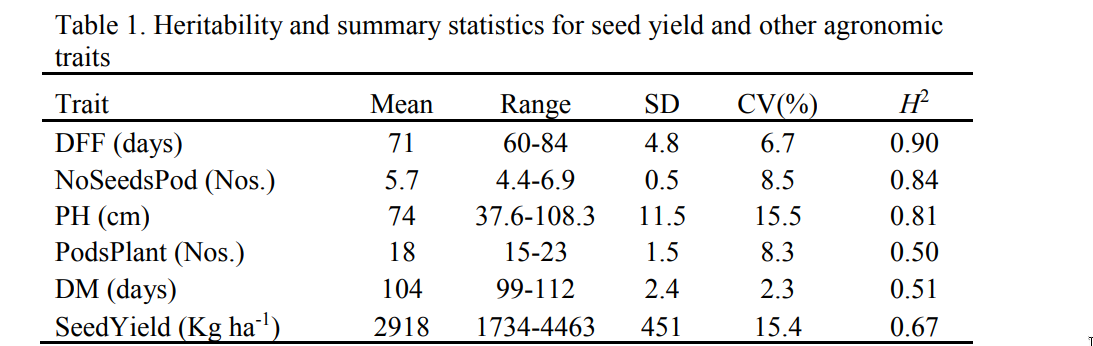
\includegraphics[width=\linewidth]{table1.png}
		{DFF is days to first flowering; NoSeedsPod is the number of seeds per pod, PH is plant height, PodsPlant is the number of pods per plant, DM is days to physiological maturity, SeedYield is seed yield per hectare, SD is the standard deviation, CV is coefficient of variance, $H^2$ is heritability in the broad sense.}
		\end{figure}
\end{center}

\subsection{Comparison of predictive ability}
\begin{center}
	\begin{figure}[H]
	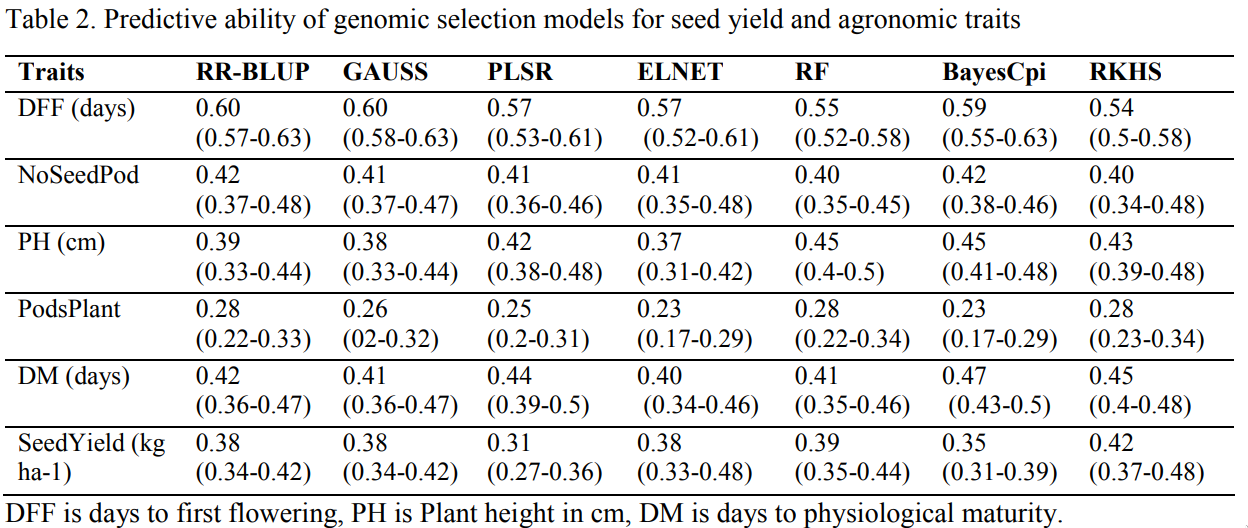
\includegraphics[width=\linewidth]{table2.png}
		\end{figure}
\end{center}


\section{VM Hardening - Security Implementation}
The following security checklist was provided to NDSU BPDM for internal improvement of virtual machines and was tested using Centos 8.

\begin{enumerate}
\def\labelenumi{\arabic{enumi}.}
\item
  Filesystem

  \begin{itemize}
  \item
    \texttt{/etc/fstab}

    \begin{itemize}
    \item
      \texttt{/tmp} mounted with `nodev,nosuid,noexec'
    \item
      \texttt{/var}, \texttt{/var/log}, and \texttt{/var/log/audit}, and
      \texttt{/home} are on seperate partitions
    \item
      bind mount \texttt{/var/tmp} to \texttt{/tmp}
    \item
      set `nodev' on \texttt{/home}
    \item
      set `nodev,nosuid,noexec' for \texttt{/dev/shm}
    \end{itemize}
  \item
    Set sticky bit on all world-writable directories
  \end{itemize}
\item
  System Updates

  \begin{itemize}
  \item
    set system to update automatically
  \item
    set proper repositories for development libraries
  \item
    reserve cron jobs for nessessary system downtime
  \end{itemize}
\item
  Secure Boot

  \begin{itemize}
  \item
    for the following directories, root ownership via \texttt{chown} and
    \texttt{chmod\ 600}

    \begin{itemize}
    \item
      \texttt{/boot/grub/grub.cfg}
    \item
      \texttt{/etc/fstab}
    \item
      \texttt{/etc/grub.conf}
    \end{itemize}
  \item
    \texttt{sed\ -i\ "/SINGLE/s/sushell/sulogin/"\ /etc/sysconfig/init}
  \item
    \texttt{sed\ -i\ "/PROMPT/s/yes/no/"\ /etc/sysconfig/init}
  \item
    set a bootloader password for UEFI subsystem
  \end{itemize}
\item
  Process Hardening

  \begin{itemize}
  \item
    Restrict Core Dumps

    \begin{itemize}
    \item
      edit \texttt{/etc/systemd/coredump.conf} and set \texttt{Storage}
      to \texttt{none} and \texttt{ProcessSizeMax} to \texttt{0}
    \item
      run \texttt{Systemctl\ daemon-reload}
    \item
      \texttt{echo\ "fs.suid\_dumpable=0"\ \textgreater{}\textgreater{}\ /etc/sysctl.conf}
    \item
      \texttt{sysctl\ -p}
    \item
      Add line \texttt{hard\ core\ 0} to
      \texttt{/etc/security/limits.conf}
    \item
      Add line \texttt{fs.suid\_dumpable\ =\ 0} to
      \texttt{/etc/sysctl.conf}
    \item
      Add line \texttt{kernel.exec-shield\ =\ 1} to
      \texttt{/etc/sysctl.conf}
    \end{itemize}
  \item
    Randomize Virtual Memory

    \begin{itemize}
    \item
      Add line \texttt{kernel.randomize\_va\_space\ =\ 2} to
      \texttt{/etc/sysctl.conf}
    \end{itemize}
  \end{itemize}
\item
  OS Hardening

  \begin{itemize}
  \item
    remove unused legacy services (rsh, rlogin, rcp, ypserv, ypbind,
    tftp, talk, etc.) if present
  \item
    disable any services and applications started by xinitd or inetd not
    utilized
  \item
    remove xinetd if not needed
  \item
    disable or remove services which would not be utilized (DNS, SNMP,
    LDAP, etc.)
  \item
    set daemon umask
  \end{itemize}
\item
  Network Security

  \begin{itemize}
  \item
    \texttt{iptables} configuration to deny ssh attempts from outside
    whitelist, drop all input not related to functional tasks, drop all
    forwarded packets, conntrack established connections
  \item
    install \texttt{fail2ban} and configure to create local ssh jail
    with \texttt{maxretry} set to 3 for root login
  \item
    \texttt{/etc/ssh/sshd\_config}

    \begin{itemize}
    \item
      \texttt{PermitRootLogin\ no} set
    \item
      \texttt{AllowUsers} whitelist
    \item
      change the default ssh port
    \item
      \texttt{PermitEmptyPasswords\ no}
    \item
      \texttt{UseRoaming\ no}
    \item
      \texttt{IgnoreRhosts\ yes}
    \item
      \texttt{HostbasedAuthentication\ no}
    \item
      \texttt{X11Forwarding\ no}
    \item
      \texttt{Ciphers\ aes192-ctr,aes256-ctr}
    \item
      \texttt{ClientAliveInterval\ 900}
    \item
      \texttt{ClientAliveCountMax\ 0}
    \item
      \texttt{UsePAM\ yes}
    \item
      \texttt{loglevel\ INFO}
    \end{itemize}
  \item
    \texttt{chown\ root:root\ /etc/ssh/sshd\_config}and
    \texttt{chown\ 600\ /etc/ssh/sshd\_config}
  \end{itemize}
\item
  Prevent evil-maid attacks

  \begin{itemize}
  \item
    edit \texttt{/etc/modprobe.d/blacklist.conf}

    \begin{itemize}
    \item
      add line \texttt{blacklist\ usb\_storage}
    \end{itemize}
  \item
    edit \texttt{/etc/rc.local}

    \begin{itemize}
    \item
      add lines: \texttt{modprobe\ -r\ usb\_storage} and
      \texttt{exit\ 0}
    \end{itemize}
  \end{itemize}
\item
  Daemon auditing

  \begin{itemize}
  \item
    The following are legacy services that should not be running or
    installed. Check for these with \texttt{apt}, \texttt{yum}, and/or
    \texttt{systemctl}

    \begin{itemize}
    \item
      Telnet
    \item
      RSH
    \item
      NIS
    \item
      TFTP
    \item
      TALK
    \end{itemize}
  \item
    The following should only be running and installed if nessessary to
    allow for work performed
  \item
    SFTP
  \item
    DNS
  \item
    LDAP
  \item
    SMB
  \item
    DHCP
  \item
    NFS
  \item
    SNMP
  \item
    HTTPD
  \item
    \texttt{grep\ umask\ /etc/init.d/functions} and ensure this is
    \texttt{027} or \texttt{022}
  \item
    \texttt{sudo\ service\ xinetd\ stop;\ sudo\ chkconfig\ xinetd\ off}
    if xinetd is not needed
  \end{itemize}
\item
  Network Params

  \begin{itemize}
  \item
    In \texttt{/etc/sysctl.conf} set the following

    \begin{itemize}
    \item
      \texttt{net.ipv4.ip\_forward\ =\ 0}
    \item
      \texttt{net.ipv4.conf.default.send\_redirects\ =\ 0}
    \item
      \texttt{net.ipv4.conf.all.accept\_redirects\ =\ 0}
    \item
      \texttt{net.ipv4.conf.default.accept\_redirects\ =\ 0}
    \item
      \texttt{net.ipv4.icmp\_ignore\_bogus\_error\_responses\ =\ 1}
    \item
      \texttt{net.ipv4.tcp\_syncookies\ =\ 1}
    \item
      \texttt{sysctl\ -p}
    \end{itemize}
  \end{itemize}
\item
  Config hardening

  \begin{itemize}
  \item
    \texttt{chmod\ 644\ /etc/passwd}
  \item
    \texttt{chown\ root:root\ /etc/passwd}
  \item
    \texttt{chmod\ 644\ /etc/group}
  \item
Drupal+Tripal+Chado stack research    \texttt{chmod\ root:root\ /etc/group}
  \item
    \texttt{chmod\ 600\ /etc/shadow}
  \item
    \texttt{chown\ root:root\ /etc/shadow}
  \item
    \texttt{chmod\ 600\ /etc/gshadow}
  \item
    \texttt{chown\ root:root\ /etc/gshadow}
  \end{itemize}
\item
  Cron Hardening

  \begin{itemize}
  \item
    \texttt{chown\ root:root\ /etc/anacrontab}
  \item
    \texttt{chmod\ og-rwx\ /etc/anacrontab}
  \item
    \texttt{chown\ root:root\ /etc/crontab}
  \item
    \texttt{chmod\ og-rwx\ /etc/crontab}
  \item
    \texttt{chown\ root:root\ /etc/cron.hourly}
  \item
    \texttt{chmod\ og-rwx\ /etc/cron.hourly}
  \item
    \texttt{chown\ root:root\ /etc/cron.daily}
  \item
    \texttt{chmod\ og-rwx\ /etc/cron.daily}
  \item
    \texttt{chown\ root:root\ /etc/cron.weekly}
  \item
    \texttt{chmod\ og-rwx\ /etc/cron.weekly}
  \item
    \texttt{chown\ root:root\ /etc/cron.monthly}
  \item
    \texttt{chmod\ og-rwx\ /etc/cron.monthly}
  \item
    \texttt{chown\ root:root\ /etc/cron.d}
  \item
    \texttt{chmod\ og-rwx\ /etc/cron.d}
  \end{itemize}
\item
  ACL and Password Policy Enforcement

  \begin{itemize}
  \item
    Enable SELinux

    \begin{itemize}
    \item
      edit \texttt{/etc/selinux/config} and set line
      \texttt{SELINUX=enforcing}
    \end{itemize}
  \item
    Enable PAM and config:

    \begin{itemize}
    \item
      \texttt{/etc/pam.d/other}
    \item
      \texttt{/etc/pam.d/common-password}
    \item
      \texttt{/etc/pam.d/password-auth}
    \item
      \texttt{/etc/pam.d/system-auth}
    \item
      \texttt{/etc/pam.d/su}
    \item
      \texttt{/etc/security/pwquality.conf}
    \end{itemize}
  \end{itemize}

\item
  Utilities

  \begin{itemize}
  \item
    Install and run \texttt{lynis}

    \begin{itemize}
    \item
      \texttt{cd\ /opt/}
    \item
      \texttt{git\ clone\ https://github.com/CISOfy/lynis}
    \item
      \texttt{cd\ lynis;\ ./lynis\ audit\ system}
    \end{itemize}
  \item
    Install and run \texttt{rkhunter}

    \begin{itemize}
    \item
      \texttt{sudo\ apt\ install\ rkhunter} or
      \texttt{yum\ install\ rkhunter}
    \item
      \texttt{rkhunter\ -c}
    \item
      \texttt{crontab\ -e} followed by
      \texttt{0\ 3\ *\ *\ *\ /usr/sbin/rkhunter\ -c\ 2\textgreater{}\&1}
    \end{itemize}
  \item
    install and run \texttt{clamav}

    \begin{itemize}
    \item
      \texttt{sudo\ apt-get\ install\ clamav} or
      \texttt{yum\ install\ clamav}
    \item
      \texttt{freshclam}
    \item
      \texttt{clamscan\ -r\ -i\ /}
    \end{itemize}
  \item
    install \texttt{ntp} server

    \begin{itemize}
    \item
      \texttt{sudo\ apt-get\ install\ ntp}
    \item
      edit \texttt{/etc/ntp.conf}such that server is set to
    \item
      \texttt{systemctl\ enable\ ntp\ \&\&\ systemctl\ restart\ ntp}
    \item
      \texttt{timedatectl\ set-ntp\ off}
    \end{itemize}
  \item
    install \texttt{syslog} daemon
  \end{itemize}
\item
  Remove uncommon protocols and filesystems from kernel
\item
  adding hidepid to /proc

  \begin{itemize}
  \item
    \texttt{mount\ -o\ remount,rw,hidepid=2\ /proc}
  \item
    \texttt{echo\ 1\ \textgreater{}\ /proc/sys/kernel.sysrq}
  \end{itemize}
\item
  banners \texttt{/etc/issue.net}

  \begin{center}\rule{0.5\linewidth}{0.5pt}\end{center}

\begin{verbatim}
                    NOTICE TO USERS
\end{verbatim}
\end{enumerate}

Attached here should be included a banner decided as proper forewarning
by NDSU ITC as a warning for unauthorized users to log off immediately
if they have not recieved prior authorization

\begin{center}\rule{0.5\linewidth}{0.5pt}\end{center}

\begin{enumerate}
\def\labelenumi{\arabic{enumi}.}
\setcounter{enumi}{16}
\item
  Make su unavailable to normal users

  \begin{itemize}
  \item
    \texttt{sudo\ dpkg-statoverride\ -\/-update\ -\/-add\ root\ sudo\ 4750\ /bin/su}
  \end{itemize}
\end{enumerate}

\section{Mediawiki Docker Container
Setup}
To begin setup, install docker. On Centos8, this is:
\texttt{dnf\ -y\ install\ docker-ce\ -\/-nobest}

configure firewall so docker containers can forward packets to each
other without issues:
\lstset{language=BASH}
\begin{lstlisting}
  firewall-cmd --permanant --zone=public --add-rich-rule='rule family=ipv4 source address=172.27.0.0/16 accept'
  firewall-cmd --reload
  sysctl net.bridge.bridge-nf-call-iptables=0
  sysctl net.bridge.bridge-nf-call-iptables=0
  sysctl net.bridge.bridge-nf-call-arptables=0
  sysctl net.bridge.bridge-nf-call-ip6tables=0
\end{lstlisting}
Pull the needed docker images and run them:
\begin{lstlisting}
docker run --name=mariadb -p 3306:3306 -v wiki-volume:/var/lib/mysql \
-e MARIADB_ROOT_PASSWORD=CHANGETHISPASS123 -d mariadb
docker run --name=wikiname -p 80:80 -p 443:443 --link maria-db \
-d simplyintricate/mediawiki
\end{lstlisting}
copy over config files, including the system .key file you generate with
a certificate signing authority - otherwise just use
\href{https://letsencrypt.org/}{letsencrypt}
\begin{lstlisting}
docker cp ./bundle.cer wikiname:/etc/nginx/conf.d/
docker cp ./yoursite.key wikiname:/etc/nginx/conf.d/
docker cp ./default.conf wikiname:/etc/nginx/conf.d/
docker restart wikiname
\end{lstlisting}

Finally, install mediawiki as per normal using the browser, but use the name of the mariadb server container as your SQL server host during installation.

\section{Acknowledgements}
	This work used resources of the Center for Computationally Assisted Science and Technology (CCAST) at North Dakota State University.

	I would like to extend my sincerest gratitude and acknowledge the contributions of Dr Nonoy Bandillo, Dr Ana Morales-Heilman, Dr Thomas Walk, Dr Md Abdullah Al Bari, Hannah M. Worral, Nick Dusek, and the other members of the research community at NDSU: their guidance, knowledge, and human warmth have made this undergraduate research experience a wonderful one.

This summer and the previous semester, I was fortunate enough to work for North Dakota State University (NDSU) with the Bandillo Lab research group, the Minot North Central Research Extension Center, and with the Breeding Pipeline Database Management team. As an undergraduate researcher, I worked closely with these teams throughout the summer and fall to improve and audit information technology systems used for agronomic phenotype data, and also to research and implement technological improvements for both the pulse crop program specifically and the plant sciences breeding pipeline system in general.

	\end{appendices}

\bibliographystyle{plain}
\bibliography{BIOL492_writeup.bib}
\addcontentsline{toc}{section}{Bibliography}

\end{document}
